%% Copyright (C) 2009 by Tobias Elze
%% Journal of Vision LaTeX template version 1.0
%% This document may be used freely for your own submissions.

\documentclass{jov}
\usepackage{graphicx} % needed for figures
\usepackage{subcaption}
\usepackage{hyperref}
\usepackage{amsmath}
\usepackage{bbm}
\usepackage{amssymb}
\usepackage{comment}

\DeclareMathOperator*{\argmin}{arg\,min}

\begin{document}

\title{Luminance constancy under fixed geometry}
\abstract{The light that reflects off an object surface and is captured by our eyes varies significantly with its context. But, the human visual system has the ability to stably perceive the object's color invariant of the context variations. The mechanism of this behaviorally significant invariance detection ability remains largely unknown. To understand the computational principles that lead to such invariant perception, we study the perception of LRV under spectral variations in 3D scenes. Specifically, we study the effects of variations in reflectance and illumination spectra in a scene on the perceived luminance of an object. We have developed a software that generates naturalistic multispectral images of 3D scenes with precise control over the geometrical and spectral properties of the constituents that make a scene. We label these images with the luminance of a specific object in the scene. Next, we simulate the response of the retinal cones to these multispectral images using an accurate model of the early visual system. We then use supervised learning methods on these labeled cone responses to identify the computations that lead to accurate luminance estimation. We show that if only either target, or background, or illumination spectra are allowed to vary, the standard luminance can be estimated through simple transformations of the cone responses. When all the spectra vary simultaneously, while it is not easy to recover the luminance through simple transformations, a decoding scheme that compares the light from the target and the surround, and properly adds the response of the L,M and S cones can recover the luminance within about 15\% RMSE.}

\author{Singh}{Vijay}
 {Computational Neuroscience Initiative}
 {and Department of Physics, University of Pennsylvania, PA, USA}
 {}{vsin@sas.upenn.edu}

\keywords{color constancy, luminance constancy, supervised learning}

\maketitle

\section{Introduction}
The perceived color of an object has important behavioral implications, since color helps to identify objects and their properties \cite{Mollon89, Jacobs81}.
[THIS PERCEIVED COLOR DEPENDS ON THE SURFACE REFLECTANCE OF THE OBJECT.]
Perceived object color is not sensed directly. Rather, it is computed by the brain starting with the retinal image of the light reflected from an object to the eye.
The computational challenge underlying object color perception is that this reflected light depends not just on the object's surface reflectance, but also on extrinsic factors such as the illumination, the object's pose, and the position of the observer (Fig.~\ref{fig:introSchematic}).
To produce a stable perceptual representation correlated with an object's surface reflectance the brain must account for these intrinsic factors on the reflected light.
The ability of a visual system to extract such a stable representation is called color constancy. 
[DO WE NEED THIS LINE -] Although human color constancy is by no means perfect, it is often very good \cite{FosterColorConstancy, BrainardColorConstancy}. 
In this paper, we consider the computational problem of color constancy, that is, how in principle could a visual system process the light reflected to the eye to produce percepts well-correlated with object surface reflectance.

Early work on computational color constancy considered a simplified case with multiple flat matte objects and a single spatially diffuse illuminant \cite{LandRetinex,Buchsbaum80,MaloneyWandell86}. Subsequent computational work considered more complex geometries and incorporated probabilistic descriptions of the statistics of naturally occurring scenes \cite{funt1988color, D'ZmuraConstancy3, barron2012color, D'ZmuraIversonSinger,BrainardFreeman}; LET'S SEE IF WE CAN FIND SOME RECENT REVIEWS).
A key insight from this computational work is that stable color descriptors of a target object cannot be obtained from the light reflected from the target object alone.  But, it is possible to obtain such descriptors by analyzing jointly the light reflected from all of the objects in the scene.
As a consequence, the performance of color constancy algorithms will be affected by variation in the surface reflectance of all of the objects in the scene \cite{BrainardWandellRetinex}, not just by variation in the illuminant. Thus evaluation of constancy algorithms must include assessment of their performance with respect to both variation in the illumination and the surface reflectance of all of the scene objects \cite{BrainardWandellRetinex,BrainardFreeman}. 

% Figure 1: Introduction
\begin{figure}
\centering
\begin{subfigure}{0.4 \textwidth}
	\centering
	\caption{}
        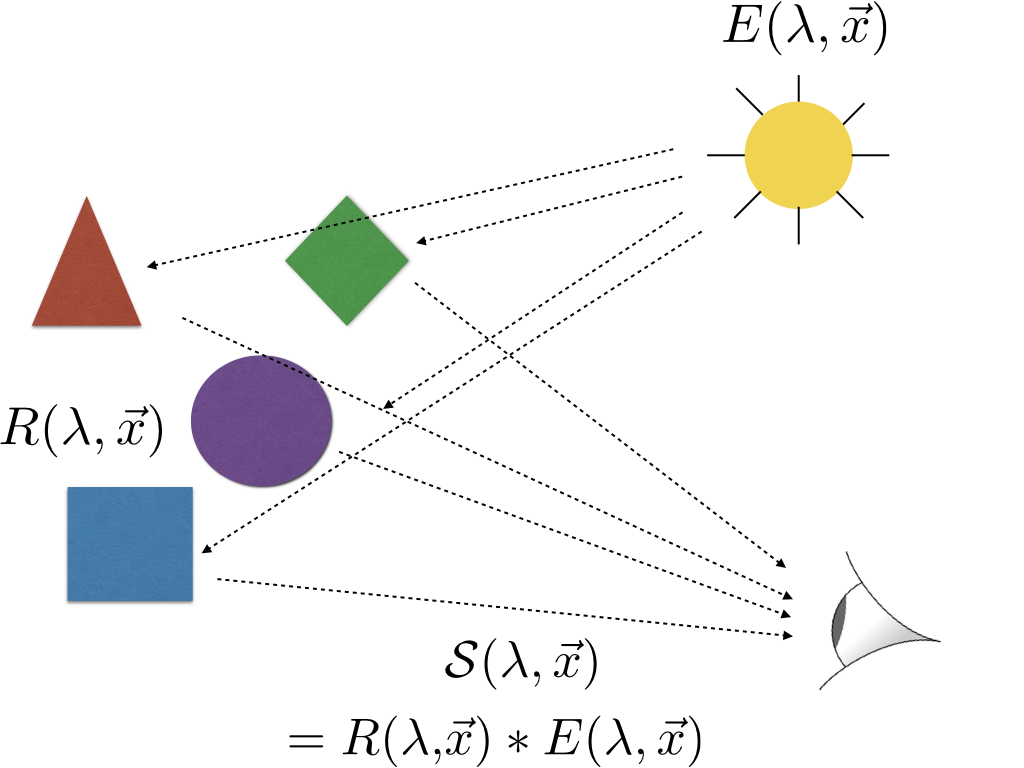
\includegraphics[width=\textwidth]{../Figures/Figure1/Figure1_a.png}
        \label{fig:introSchematic}
    \end{subfigure}
    \begin{subfigure}{0.55 \textwidth}   
        \caption{}    
        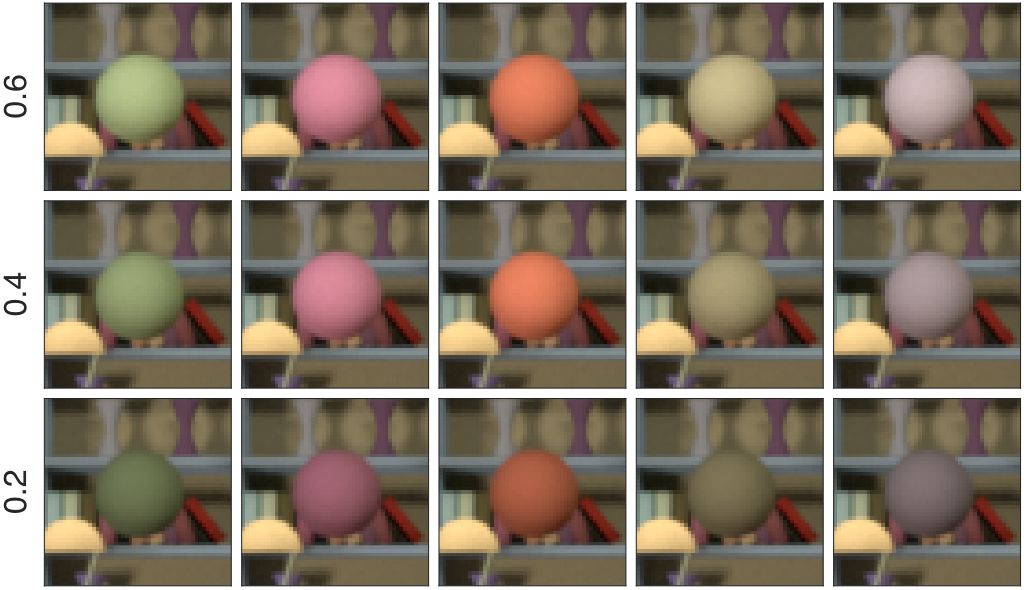
\includegraphics[width=\textwidth]{../Figures/Figure1/Figure1_b.png}
        \label{fig:introExampleFigure}
    \end{subfigure}
    \label{introFigure}
    \caption{(a) {\bf Color Constancy:} The light reflected from an object to the eye depends both on the object's surface reflectance of the object and the illumination. It also depends on geometric factors, such as the object's shape, pose, and position relative to the observer. The human visual system is able to account for variations in the reflected light due to object-extrinsic factors and produce a percept of object color that is relatively stable, an ability called color constancy. (b) {\bf Luminance Constancy:} Images of a sphere under a fixed illuminant.  Down each column, the reflectance function of the sphere varies only by a scale factor; the relative reflectance spectrum held fixed.  The relative spectrum (shape of reflectance spectrum) varies across each row.
Within each row, the light reflectance value (LRV) of the spheres is constant. The values on the left of each row provide the corresponding LRV. We cast the problem of computational luminance constancy to be that of estimating LRV from the image, across variation in other scene factors: variation in relative surface reflectance, variation in illumination, and variation in the reflectance of the other objects in the scene.}
 \end{figure}

An alternative approach to computational color constancy, which has been less-well explored, is to use supervised machine learning techniques to develop mappings between input images and stable color descriptors \cite{barron2015convolutional}. The use of supervised learning to understand perceptual capabilities for natural stimuli has enjoyed success in domains outside of color vision. For example, a recently developed technique called accuracy maximization analysis (AMA) learns linear filters optimized for particular perceptual tasks \cite{geisler2009optimal}. It has been used to develop ideal observers for speed, focus error, and disparity estimation that provide excellent models of human performance \cite{burge2011optimal, burge2014optimal, burge2015optimal}. In this paper, we apply AMA to a special case of computational color constancy. 

Supervised learning requires large labeled data sets.  Such data sets are not readily available for the study of color constancy. Although there are databases of calibrated color images, these do not provide ground truth information about surface reflectance and illuminantion at each image location \cite{ChakrabartiHyperspectral,NascimentoFoster2016,ParragaHyperspectralData,TkacikUpennHypersepctralData,skauli2013collection,olmos2004biologically}. There are some smaller databases consisting of images of posed scenes where object surface reflectances are measured individually (\citeNP{funt1988color,ciurea2003large}; \citeauthor{davidPennHyperspectral}), but these are not large enough to drive supervised learning.
 
% Figure 2: Conditions Studied
\begin{figure}
\centering
	\begin{subfigure}[b]{0.33 \textwidth}
		\caption{Condition 2}
		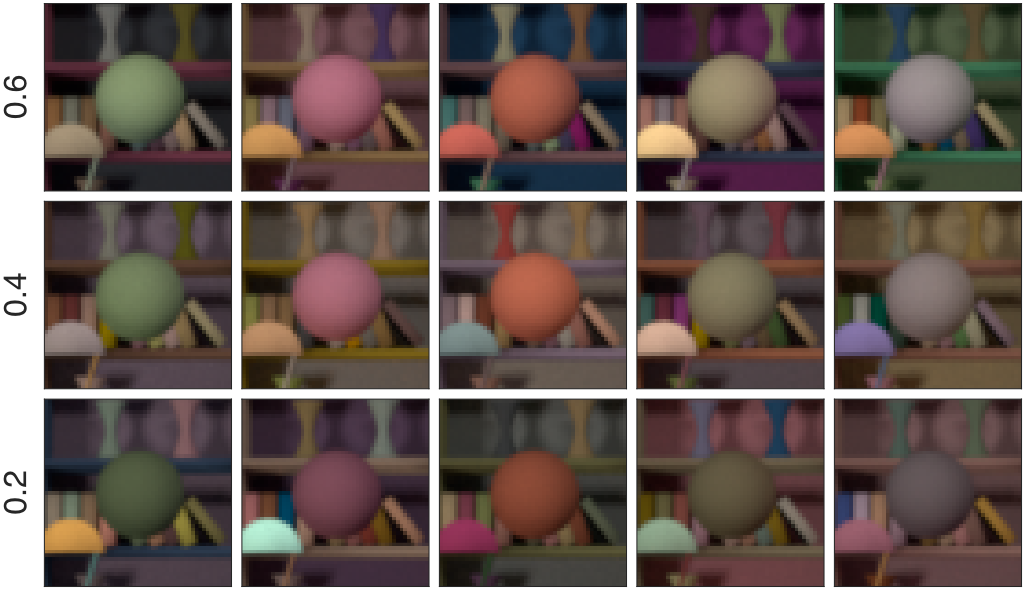
\includegraphics[width=\textwidth]{../Figures/Figure2/Figure2_a.png}
 		\label{fig:backgroundVarying}
	\end{subfigure}
	\begin{subfigure}[b]{0.33 \textwidth}
        \caption{Condition 3}	
        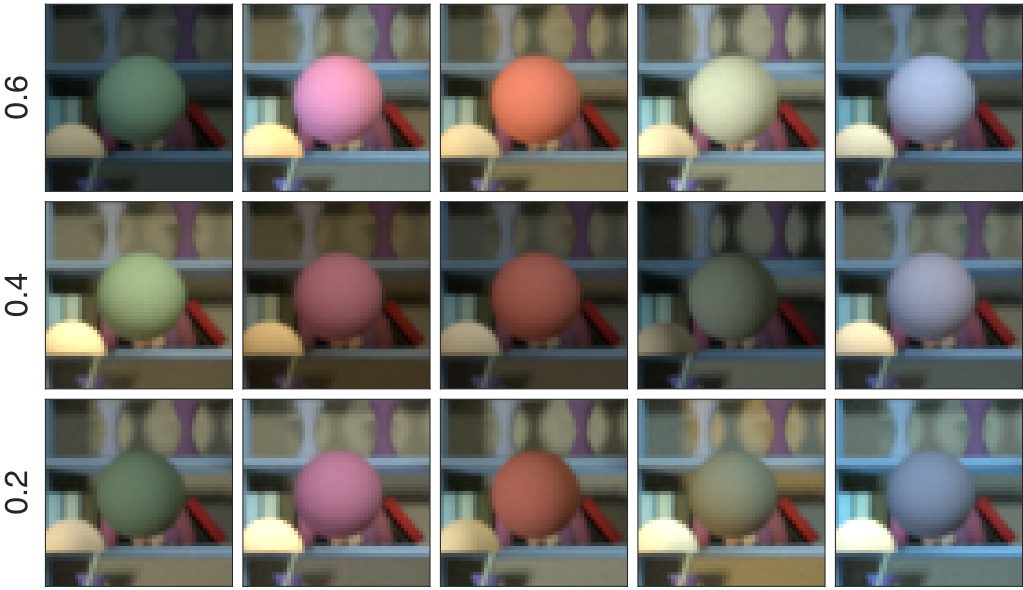
\includegraphics[width=\textwidth]{../Figures/Figure2/Figure2_b.png}
        \label{fig:targetIlluminantVarying}
    \end{subfigure}
	\begin{subfigure}[b]{0.33 \textwidth}
	\caption{Condition 4}	
        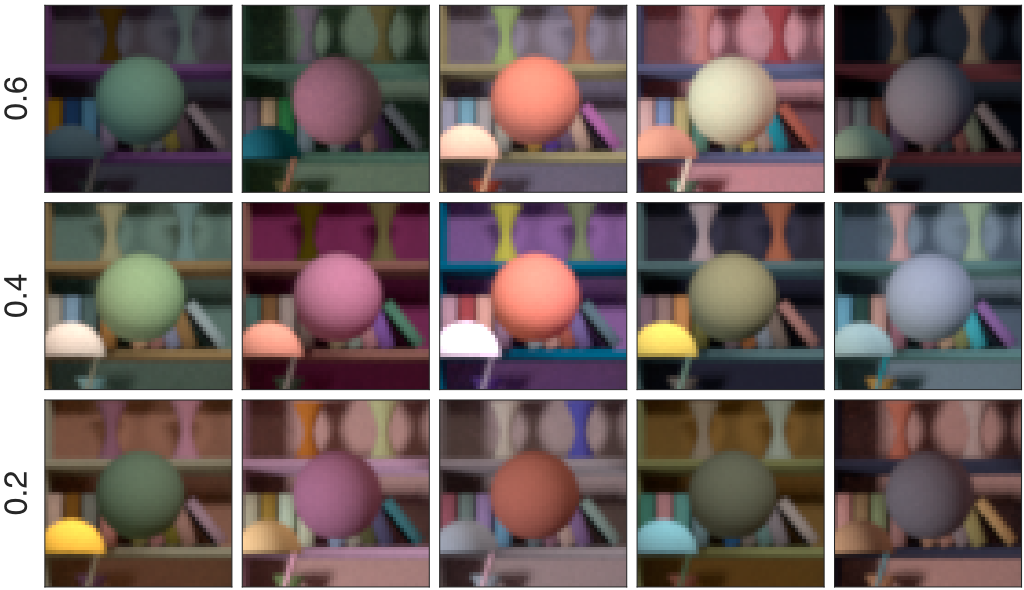
\includegraphics[width=\textwidth]{../Figures/Figure2/Figure2_c.png}        
        \label{fig:allSpectraVarying}
    \end{subfigure}    
    \caption{{\bf Types of spectral variations studied in this work:} sRGB rendition of multispectral images similar to ones studied in our work. The numbers on the left indicate the standard luminance level of the target object. 5 images are shown at each luminance level. We studied four types of spectral variations. Condition 1: target object relative surface reflectance spectrum variable, light source spectra fixed, background object spectra fixed, (Fig.~\ref{fig:introExampleFigure}). (a) Condition 2: target object relative surface reflectance spectrum variable, light source spectra fixed, background object spectra variable, (b) Condition 3: target object relative surface reflectance spectrum variable, light source spectra variable, background object spectra fixed, (c) Condition 4: target object relative surface reflectance spectrum variable, light source spectra variable, background object spectra variable. As in Fig.~\ref{fig:introExampleFigure}, the spheres in each row of each panel have the same surface luminance, while the spheres in each column of each panel have the same relative surface reflectance.  Moreover, across the four panels (Fig.~\ref{fig:introExampleFigure} \& Fig.~\ref{fig:studiedCases}), spheres in corresponding locations have the same surface reflectance. In all four panels, the overall lights source spectra scale factors (see \nameref{Methods}) were drawn from a uniform distribution on the range [0.5, 1.5]. The sRGB values for all three panels were normalized using a common scale factor prior to gamma correction.} 
\label{fig:studiedCases}
\end{figure}

In this paper, we use high-quality computer graphics to generate large data sets of naturalistic images where the surface reflectance and illumination corresponding to each image pixel are known. 
This approach allows us to investigate computational color constancy with naturalistic stimuli, while retaining the ability to control the properties of objects and illuminants. Here, we use this approach to tackle luminance constancy, a constitutive component of the more general color constancy problem (Fig.~\ref{fig:introExampleFigure}). 

% I found the definition of light reflectance value on the web, sort of.  Need to find the right citable reference and or a term for the same thing that
% we can find a reference for.
We define the computational problem of luminance constancy as that of estimating the light reflectance value (LRV) of an object's surface reflectance function.
The LRV is a measure of the overall amount of light reflected by a surface (\citeauthor{astm1121477}).
More precisely, the LRV is the luminance of the light that would
be reflected to the eye from an object with the specified surface reflectance function when the object is illuminated by a reference illuminant,
normalized by the luminance of the reference illuminant itself.
Here we use CIE daylight D65 as the reference illuminant and the CIE 1931 photopic luminosity function \cite{CIE86}.
LRVs are typically expressed in percent, so that they range from 0 to 100.

% MOVE THIS TO DISCUSSION
%This general approach has been adopted by other labs for the study of computational estimation of optical flow (Baker et al., 2011) and is becoming increasingly popular (Kovacs, Bell, Snavely, & Bala, 2017), as well as for the generation of stimuli for the study of human perception (e.g., Boyaci, Maloney, & Hersh, 2003; Todd & Mingolla, 1983; Arend & Reeves, 1986; Johnston, Cumming, & Parker, 1993). Of course, success within the domain of graphics images does not guarantee smooth generalization to real natural images, a point we return to in the Discussion.
% \cite{baker2011database}  \cite{kovacs17shading} \citeNP{boyaci2003effect, todd1983perception, arend1986Simultaneous, johnston1993integration}
% Autonmous vehicle work - ask BAW

% NOT SURE WE NEED ANY OF THIS.  PROBABLY NOT HERE IF WE DO
%Even within the special case of luminance constancy, there are many scene manipulations that could be considered. The set of manipulations we focus on here are illustrated by Fig.~\ref{fig:introExampleFigure} and the three panels of Fig.~\ref{fig:studiedCases}. These conditions are: 1. variation in target object spectrum with fixed light source and background objects spectra (Fig.~\ref{fig:introExampleFigure}), 2. variation in target object spectrum and background objects spectra, with fixed light source  (Fig.~\ref{fig:backgroundVarying}), 3. variations in both the target object spectrum and the light source spectra, with fixed background object spectra (Fig.~\ref{fig:targetIlluminantVarying}), and 3. variations in all three types of spectra (target object, light source, and background objects) (Fig.~\ref{fig:allSpectraVarying}). Across real scenes, there will also be variations in the shape of the target object, its pose, eye position, etc. (see \nameref{Methods}). In this paper, we focus on the problem of luminance constancy within scene ensembles where these geometric factors are held fixed.
%
%We show that for conditions that have spectral variation only either in target object surface reflectance or background object surface reflectance or the power spectrum of the light sources, luminance can be estimated by simple transformations of the cone responses. For variations only in target object reflectance spectra (Condition 1) or just the target and background objects reflectance spectra (Condition 2), LRV can be recovered directly from the light reflected off the target object. For Condition 3, where both the target object reflectance and light source spectra vary, LRV can be recovered from the contrast between the target and the background. When all the spectral features in the scene are allowed to change (Condition 4), the standard luminance can not be recovered simply from the cone response or the contrast. We have used AMA with a Bayesian estimator to estimate standard luminance of the target object. Using this method, we can recover the luminance of the target object with $\sim 15\%$ relative root mean square error.  Our analysis shows that the optimal receptive fields for estimating the luminance of the target object show a center surround structure, supporting a comparison between the light coming from the target object and its surround. Additionally, luminance estimation involves a weighted sum of the L, M and S cone responses where the receptive fields give more weight to the L and M cone responses compared to S cone responses. Comparing the performance of the RFs learnt using  one condition on the cone response of other conditions shows that the receptive field of the complex conditions perform well on images of simpler conditions. We discuss the implications of such receptive fields on luminance constancy. 

\section*{Methods} \label{Methods}
\subsection{Overview}
There are four key parts to our methods.  First we generate a labeled set of training images.  Second we use a model of the early visual system the compute the responses of the cone photoreceptor mosaic to the labeled images. Third we apply AMA to the cone responses to learn task-optimal receptive fields (RFs). Fourth we evaluate how well the responses of the RFs may be decoded to achieve luminance constancy.

\subsection{Labeled training data} \label{method:VirtualWorld}
% Figure 3
\begin{figure}[t]
\centering
\begin{subfigure}[b]{0.22 \textwidth}
        \caption{Library }
        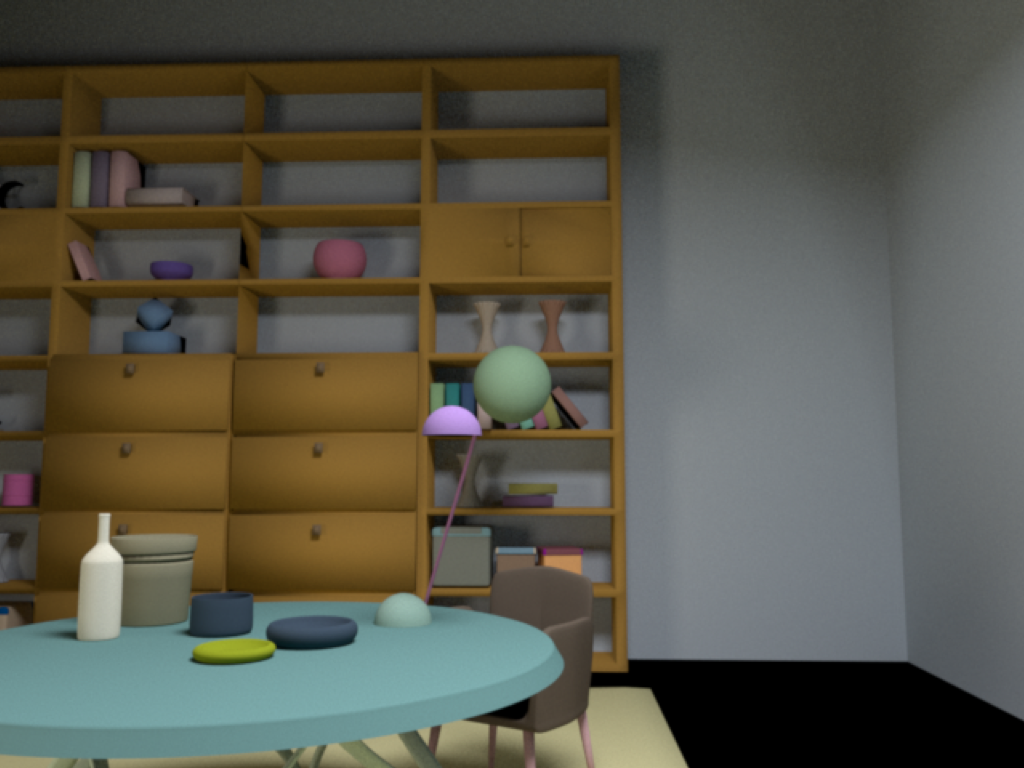
\includegraphics[width=\textwidth]{../Figures/Figure3/Figure3_a.png}
        \label{fig:baseSceneLibrary}
    \end{subfigure}
    ~
    \begin{subfigure}[b]{0.22 \textwidth}
        \caption{Mill}    
        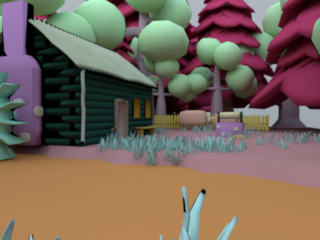
\includegraphics[width=\textwidth]{../Figures/Figure3/Figure3_b.png}
        \label{fig:baseSceneMill}
    \end{subfigure}    
    ~
    \begin{subfigure}[b]{0.22 \textwidth}
        \caption{Table-Chairs}    
        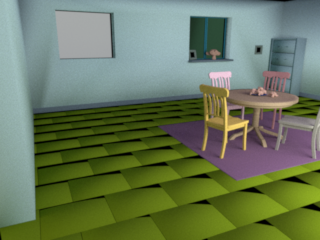
\includegraphics[width=\textwidth]{../Figures/Figure3/Figure3_c.png}
        \label{fig:baseSceneTableChairs}
    \end{subfigure}
    
    \begin{subfigure}[b]{0.22 \textwidth}
        \caption{Indoor-plant}    
        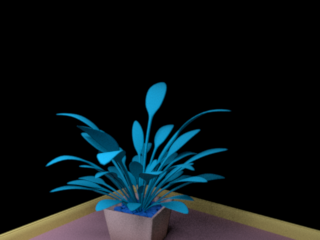
\includegraphics[width=\textwidth]{../Figures/Figure3/Figure3_d.png}
        \label{fig:baseSceneIndoorPlant}
    \end{subfigure}    
    ~
    \begin{subfigure}[b]{0.22 \textwidth}
        \caption{Warehouse}    
        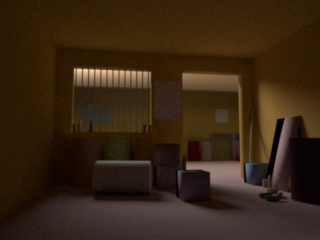
\includegraphics[width=\textwidth]{../Figures/Figure3/Figure3_e.png}
        \label{fig:baseSceneWarehouse}
    \end{subfigure}
    ~
    \begin{subfigure}[b]{0.22 \textwidth}
        \caption{Checkerboard}    
        
\includegraphics[width=\textwidth]{../Figures/Figure3/Figure3_f.png}
        \label{fig:baseSceneCheckerBoard}
    \end{subfigure}
    \caption{{\bf Example of base scenes form the VWCC library.} Each panel shows a rendering of one tamed base scene without additional objects inserted.  The reflectance spectra of the distinct surfaces in each scene has been assigned randomly (see below) using the VWCC software.  The light source spectra were also assigned randomly to the default and inserted light source.}\label{fig:baseScenes}
\end{figure}

\subsubsection{Virtual naturalistic scenes}

The light that reflects from objects to the eyes depends on many factors.
These include the surface reflectance, texture, material and geometry of the objects, the spectra of the illuminants, and the position of the observer.
We developed a rendering package (\href{https://github.com/BrainardLab/VirtualWorldColorConstancy}{Virtual World Color Constancy}, \href{http://rendertoolbox.org}{RenderToolbox4} \cite{heasly2014rendertoolbox3}) that allows us to construct models of naturalistic scenes, with key scene factors under programmatic control.
The package harnesses an open-source computer graphics renderer  \cite{jakob2015mitsuba} to produce physically-accurate images from the scene models.
Because each image is rendered from a known scene model, each image pixel can be labeled with the surface reflectance of the corresponding scene object.
By incorporating statistical models of the variation of object surface reflectance and daylight illumination, the pipeline allows us to produce large labeled sets of images that capture much of the task-relevant statistical structure of natural scenes.

% Figure 4
\begin{figure}
\centering
\begin{subfigure}[b]{0.14 \textwidth}
        \caption{Big-ball}
        
\includegraphics[width=\textwidth]{../Figures/Figure4/Figure4_a.png}
        \label{fig:libraryWithBigBall}
    \end{subfigure}
    ~ 
\begin{subfigure}[b]{0.14 \textwidth}
        \caption{Small-ball}
        
\includegraphics[width=\textwidth]{../Figures/Figure4/Figure4_b.png}
        \label{fig:libraryWithSmallBall}
    \end{subfigure}
    ~ 
    \begin{subfigure}[b]{0.14 \textwidth}
        \caption{Barrel}
        
\includegraphics[width=\textwidth]{../Figures/Figure4/Figure4_c.png}
        \label{fig:libraryWithBarrel}
    \end{subfigure}
    \begin{subfigure}[b]{0.14 \textwidth}
        \caption{Xylophone}
        
\includegraphics[width=\textwidth]{../Figures/Figure4/Figure4_d.png}
        \label{fig:libraryWithXylophone}
    \end{subfigure}
    ~
	\begin{subfigure}[b]{0.14 \textwidth}
        \caption{Ring toy}
        
\includegraphics[width=\textwidth]{../Figures/Figure4/Figure4_e.png}
        \label{fig:libraryWithRingToy}
    \end{subfigure}
        ~
    	\begin{subfigure}[b]{0.14 \textwidth}
        \caption{Bottle}
        
\includegraphics[width=\textwidth]{../Figures/Figure4/Figure4_f.png}
        \label{fig:libraryWithChampagneBottle}
    \end{subfigure}
\caption{{\bf Library base scene with inserted objects.} The rendering package was used to insert different objects into the library base scene, with each panel showing a different object. The objects were inserted at a location in the image and then the camera was pointed at the object, so that the object's image is at the center of the rendered image.  In the figure panels, the full rendered image is cropped so that the inserted object is more visually salient. We use this capability of our software pipeline to insert target objects into scenes.}\label{fig:libraryWithTarget}
\end{figure}

Our rendering package includes a collection of base scenes (Fig.~\ref{fig:baseScenes}).
Base scenes specify an arrangement of objects and light sources.
Base scenes may be enriched by the insertion of additional objects, chosen from an object library (Fig.~\ref{fig:libraryWithTarget}).
Once the position, size and pose of the inserted objects has been set, our package allows the assignment of a surface reflectance function to each object in the scene and a spectral power distribution to each light source (Fig.~\ref{fig:VWCCTransformations}).
This provides a complete scene model which can be rendered from any specified viewpoint.

% Figure5
\begin{figure}
	\begin{subfigure}[b]{0.18 \textwidth}
    \centering
        \caption{Target position}
        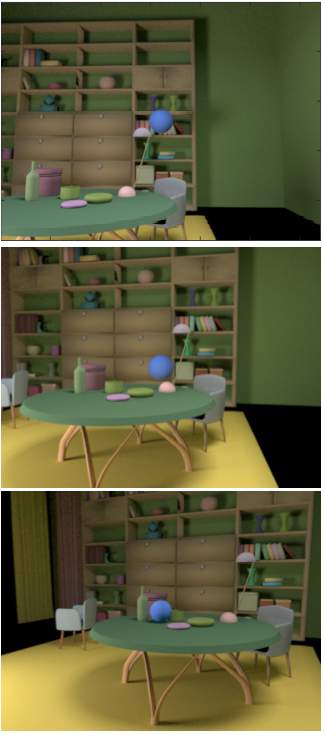
\includegraphics[width=\textwidth]{../Figures/Figure5/Figure5_d.png}
        \label{fig:targetPositionVariation}
    \end{subfigure}
    ~
	\begin{subfigure}[b]{0.18 \textwidth}
    \centering
        \caption{Target Size/Orientation}
        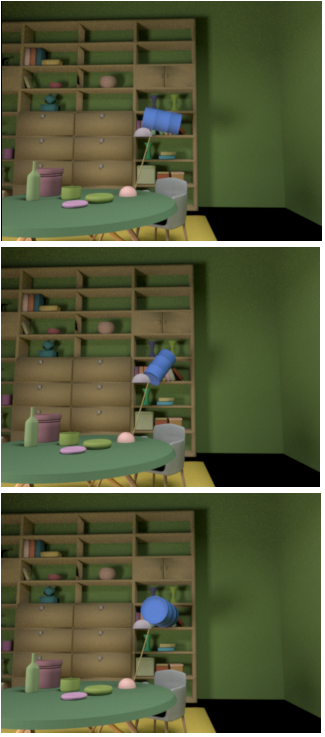
\includegraphics[width=\textwidth]{../Figures/Figure5/Figure5_e.png}
        \label{fig:targetSizeOrientation}
    \end{subfigure}
~
\centering
	\begin{subfigure}[b]{0.18 \textwidth}
    \centering
        \caption{Target spectra}
        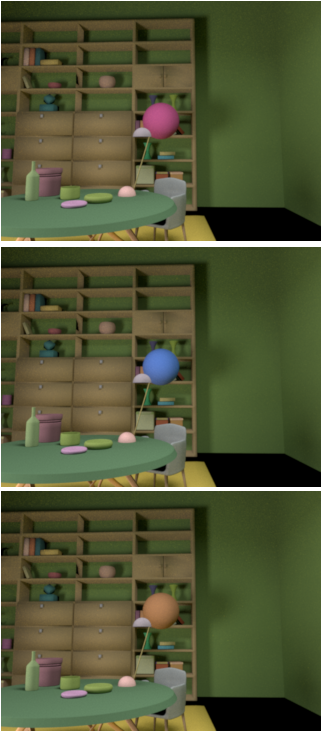
\includegraphics[width=\textwidth]{../Figures/Figure5/Figure5_a.png}
        \label{fig:targetVariation}
    \end{subfigure}
    ~
    \begin{subfigure}[b]{0.18 \textwidth}
    \centering
        \caption{Background spectra}
        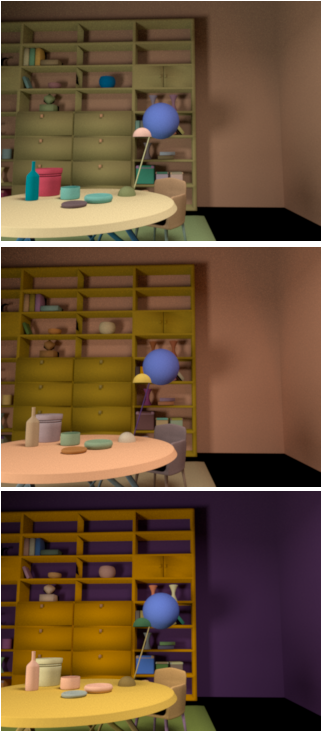
\includegraphics[width=\textwidth]{../Figures/Figure5/Figure5_b.png}
        \label{fig:backGroundVariation}
    \end{subfigure}
    ~
    \begin{subfigure}[b]{0.18 \textwidth}
    \centering
        \caption{Illumination spectra}
        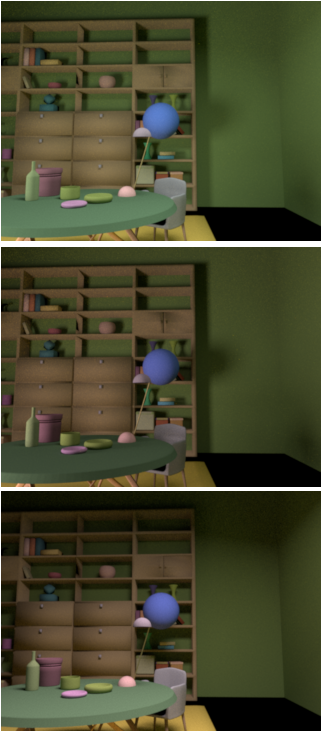
\includegraphics[width=\textwidth]{../Figures/Figure5/Figure5_c.png}
        \label{fig:illuminationVariation}
    \end{subfigure}
    \caption{{\bf Transformations of the scene.} The possible transformations of the properties of a scene can broadly be classified into two groups: Geometrical (a-b) and Spectral (c-e). VWCC provides control over such transformation as illustrated by the columns. (a) The three panels in the column have the target object at three different positions. The camera points to the center of the pixel. (b) The target object in the three panels are at different orientations. (c) The target object surface reflectance varies across the three panels of the column. (d) The surface reflectance of the background objects varies across the three panels. In each panel, the reflectances were assigned randomly. (e) The power spectrum of the light sources were assigned randomly in the three panels. 
\label{fig:VWCCTransformations}}
\end{figure}

In the present work, we used our package to generate datasets of naturalistic scenes and corresponding images.
We used one fixed base scene and inserted a target object of fixed shape and size into this scene.
We generated five distinct datasets: Conditions 0 through 4.
Across these datasets the luminance constancy problem, estimating the target object LRV,
becomes progressively more difficult (Fig.~\ref{fig:studiedCases}).
Each dataset consisted of 1000 scenes and corresponding images.

In Condition 0, the only source of stimulus variation was in the task relevant quantity, the target object LRV.
Here, we fixed target object color (i.e. the relative reflectance spectrum of the target object),
the reflectance spectra of the background objects, and the spectral power distributions of the light sources.
We used 10 LRV values, equally spaced between 20 and 60.
Condition 0 defines a baseline. In this condition, all images with the the same value of the LRV are identical.

In the remaining conditions, we systematically introduced variation in scene factors other than the target object LRV.
In Condition 1, we introduced variation in target object color but held the other factors fixed.

Conditions 2, 3 and 4 each increase the variation relative to Condition 1.
In Condition 2, in addition to the color of the target object,
we varied the reflectance spectra of the background objects
while holding the the spectral power distribution of the light sources
constant.
In Condition 3, in addition to the color of the target object,
we varied the spectral power distribution of the light sources
while holding the reflectance spectra of the background objects constant.
Finally, in Condition 4 we varied all three factors (target object color,
reflectance spectra of the background objects, spectral power distribution of the light sources).
The variation within our datasets captures the essence of the computational problem of lightness constancy
up to effects of scene geometry, an additional richness that we do not address in this paper.

% 1000 each Condition
%Condition 0: Baseline
%Condition 1: Target Color Only Variation
%Condition 2: Target Color and Background
%Condition 3: Target Color and Illuminant
%Condition 4a: Target Color, Background and Relative Illuminant
%Condition 4: Everything

For the primary results, we used the ``{\it Library}'' base scene and a spherical target object .
The library base scene contains X area lights. We inserted one additional spherical spherical light source into the scene.
The position and size of the inserted object, inserted light source and viewpoint were held fixed across all scenes in the database,
as shown in Figure~\ref{fig:3DScene}.
Surface and illuminant spectra were drawn according to statistical models of naturally occurring spectra.
We describe these models below.
Multispectral images ($320 \times 240$ pixels) were rendered at 31 evenly-spaced wavelengths between $400$nm and $700$nm.

%Once a base scene has been chosen and objects and light sources inserted, we assign spectral surface reflectance, texture, and material property to each object surface in the scene. We also assign an illuminant spectral power distribution to each light source in the scene. Objects in the VWCC library may contain more than one distinct surface, each of which may be assigned a different surface reflectance. As with object position, these may be specified programatically. In the present work, we use simple choices for texture (all surfaces spatially uniform) and material property (all surfaces matte) and focus on variation in surface spectral reflectance. 

% REMOVE PANELS A AND D AND FIX CAPTION AND REFERENCES TO THIS FIGURE.
\subsubsection{Illumination spectra}
% Figure 6
\begin{figure}
\centering
    \begin{subfigure}[b]{0.24 \textwidth}
    \centering
	\caption{}
        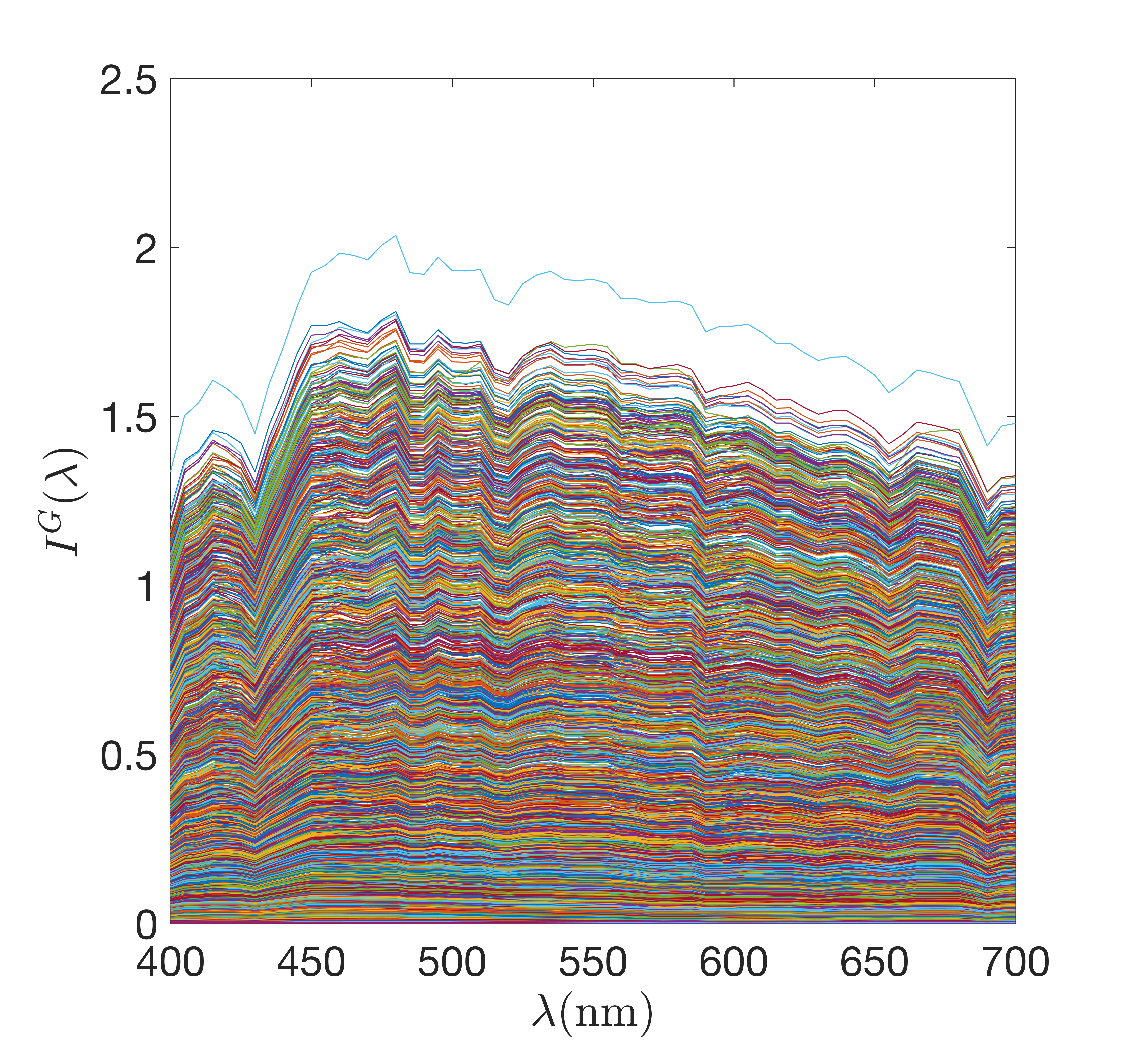
\includegraphics[width=\textwidth]{../Figures/Figure6/Figure6_a.pdf}
        \label{fig:granadaData}
    \end{subfigure}
	\begin{subfigure}[b]{0.24 \textwidth}
    \centering
        \caption{}
        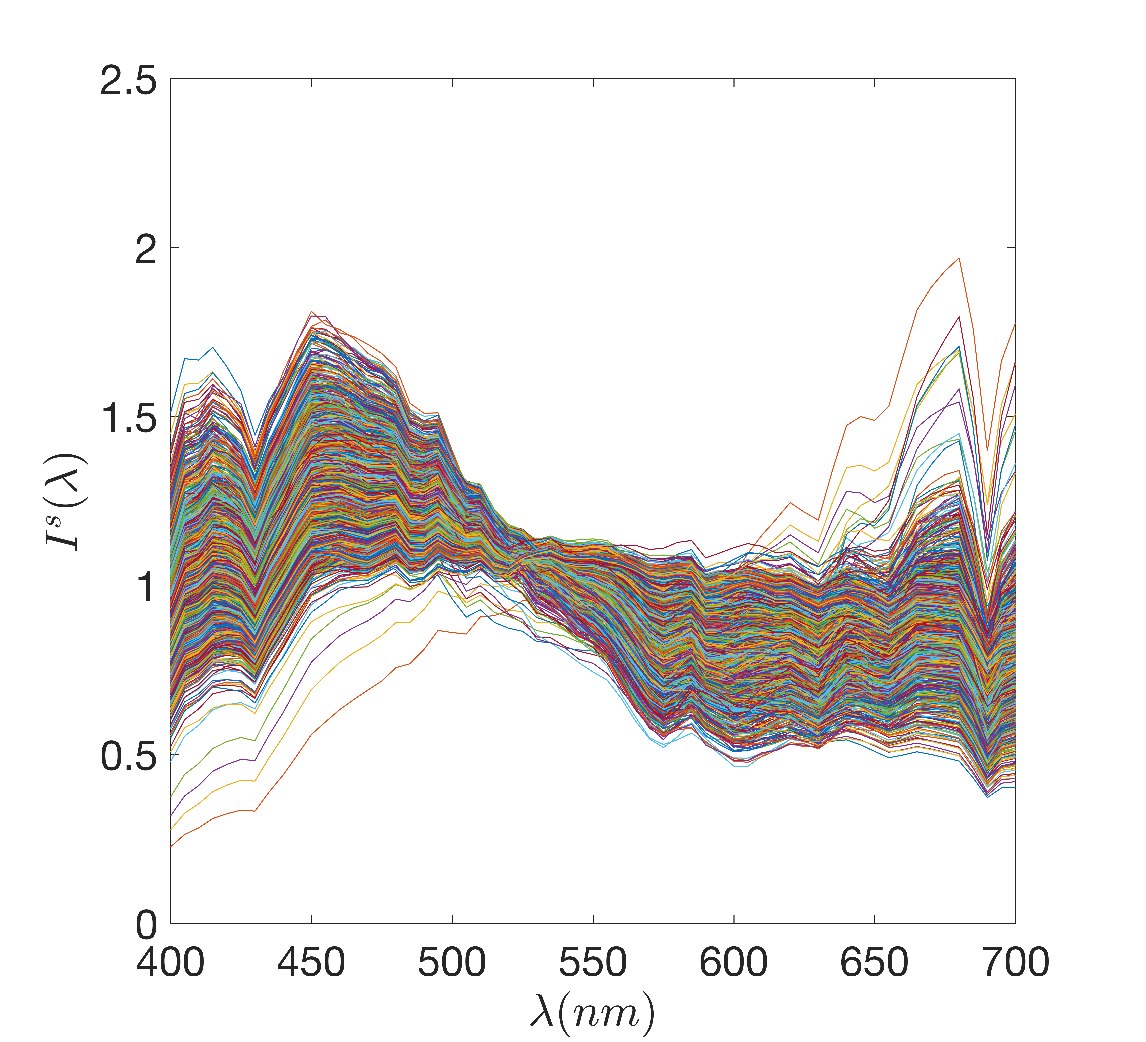
\includegraphics[width=\textwidth]{../Figures/Figure6/Figure6_b.pdf}
        \label{fig:illuminantSamples}
    \end{subfigure}
      	\begin{subfigure}[b]{0.24 \textwidth}
    \centering
        \caption{}
        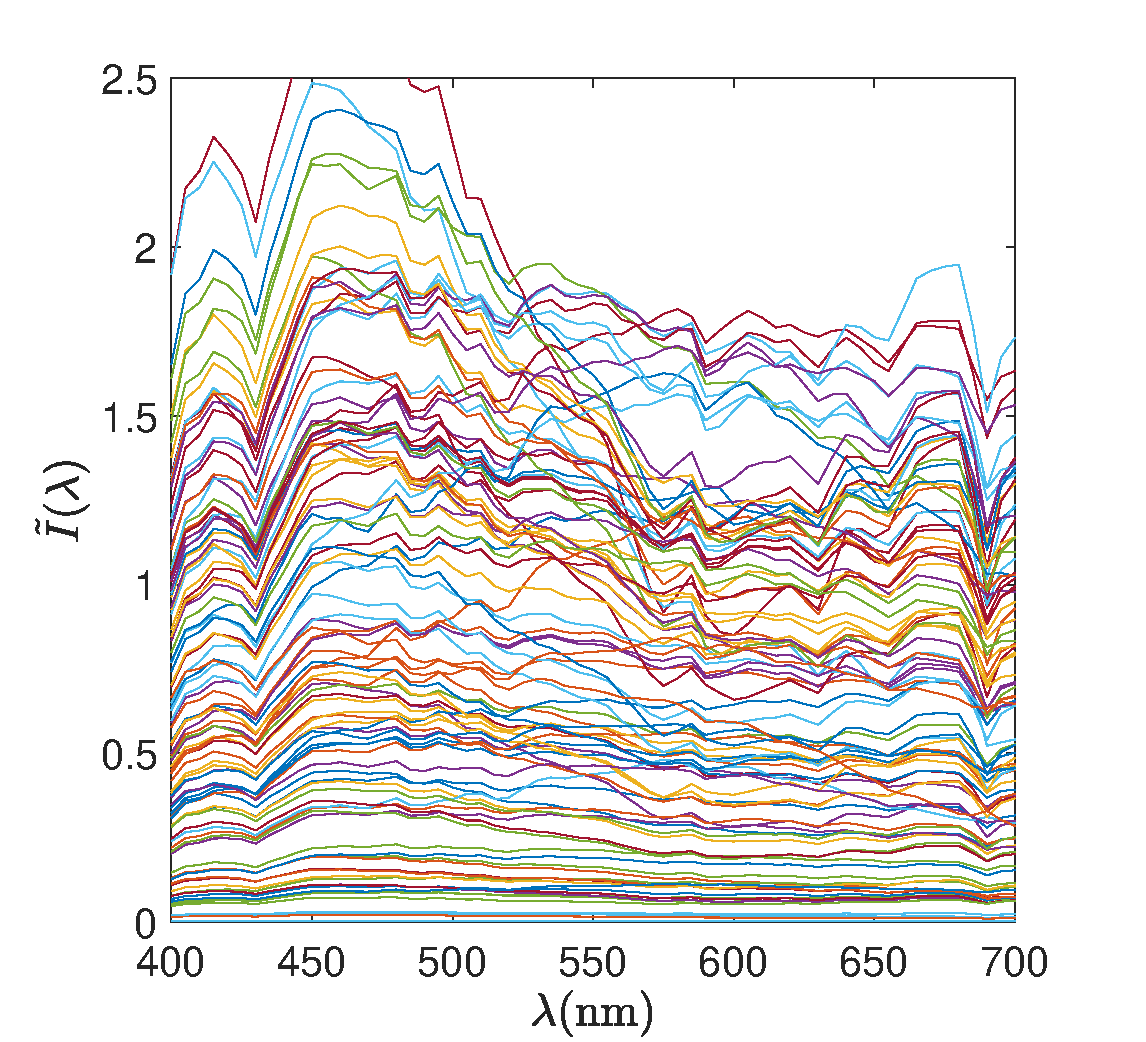
\includegraphics[width=\textwidth]{../Figures/Figure6/Figure6_c.pdf}
        \label{fig:xyDiagram}
        \end{subfigure}
      	\begin{subfigure}[b]{0.24 \textwidth}
    \centering
        \caption{}
        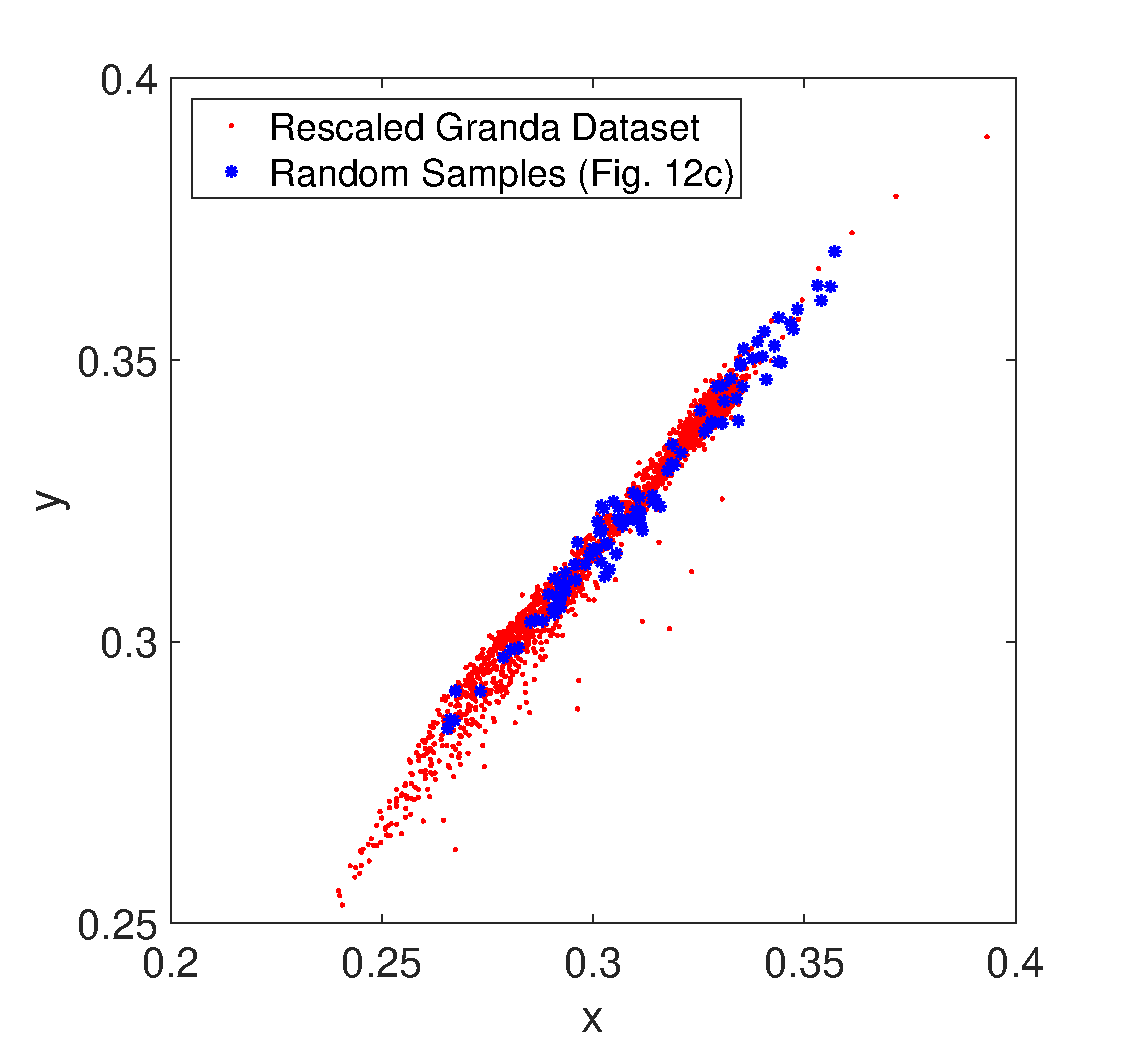
\includegraphics[width=\textwidth]{../Figures/Figure6/Figure6_d.pdf}
        \label{fig:sRGBIlluminant}
    \end{subfigure}
    \caption{{\bf Illumination spectra:} (a) Granada dataset. The spectra are normalized by the mean over wavelength. (b) A representative sample of spectra generated using normalized Granada dataset. (c) CIE xy chromaticity diagram of the normalized dataset and the random samples. (d) sRGB renditions of the samples from Figure~\ref{fig:illuminantSamples}.}
\label{fig:illuminant}
\end{figure}

To generate illumination spectra, we developed a statistical model of the \href{http://colorimaginglab.ugr.es/pages/Data}{Granada daylight measurements} \cite{peyvandi2016colorimetric} and sample randomly from the model.
The overall intensity of the measurements spans approximately three orders of magnitude.
Figure~\ref{fig:granadaData} plots the measurements in normalized form to make apparent the variation in the relative spectra. The spectra are normalized by their mean over wavelength.

Our statistical model approximates these normalized shapes using their first 6 principle components, and models the variation in these components with
a 6-dimensional Gaussian whose mean and covariance matrix match the dataset's sample mean and covariance of the weights on these components \cite{BrainardFreeman}.
To generate a random relative illuminant spectrum, we take a draw from this Gaussian to obtain weights and generate the corresponding spectrum.
Figure~\ref{fig:illuminantSamples} illustrates the relative spectra of draws obtained using this procedure.
Details of the statistical model for illumination are provided in the appendix.

Because our multivariate Gaussian model is based on the rescaled spectra, it does not embody the large variation in overall intensity of natural daylights.
To obtain illuminant spectra with intensity variation similar to the Granada dataset, we scaled each randomly generated relative spectrum.
We obtained each scale factor by randomly sampling (with replacement) a spectrum from the Granda dataset and taking its mean. 
Color swatches of samples of illuminant spectra are shown in Figure~\ref{fig:sRGBIlluminant}.

% Fix case in headers to sentence style, here and elsewhere
\subsubsection{Surface reflectance spectra}
% Figure 7
\begin{figure}
\centering
	\begin{subfigure}{0.24 \textwidth}
    \centering
            \caption{}
        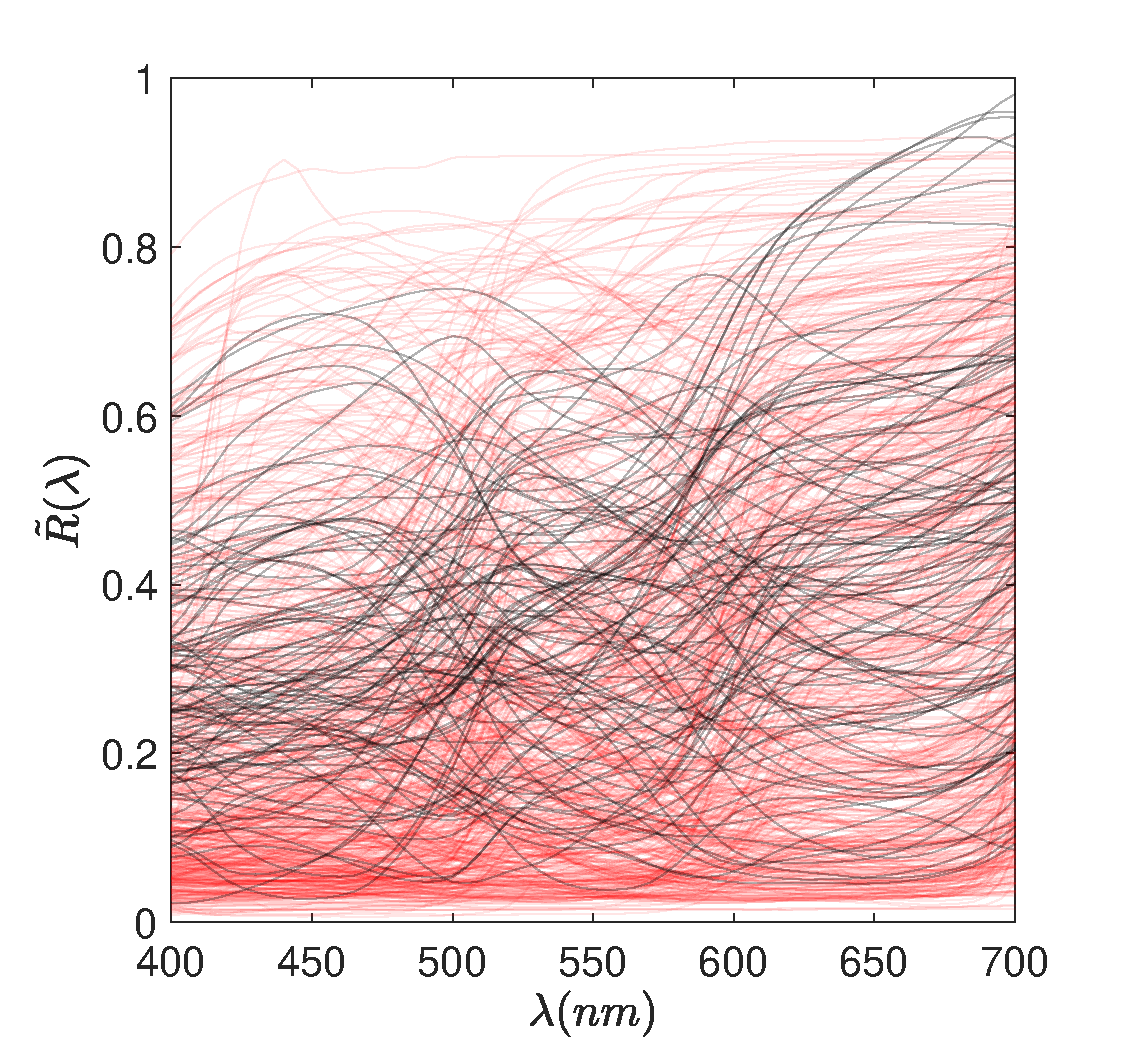
\includegraphics[width=\textwidth]{../Figures/Figure7/Figure7_a.pdf}
        \label{fig:reflectanceSpectra}
    \end{subfigure}
    \begin{subfigure}{0.24 \textwidth}
    \centering
        \caption{}
        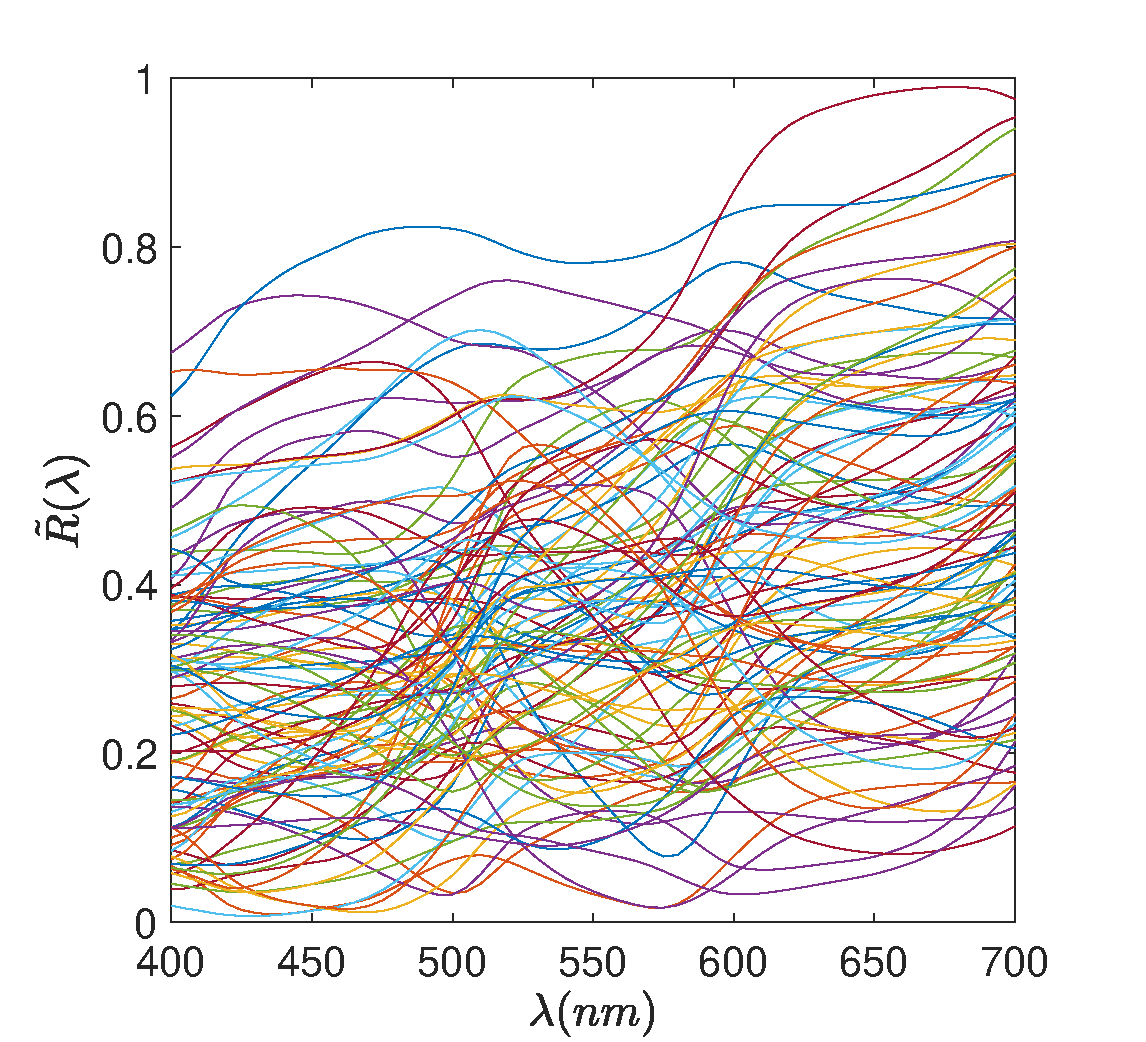
\includegraphics[width=\textwidth]{../Figures/Figure7/Figure7_b.pdf}
        \label{fig:reflectanceSamples}
    \end{subfigure}
    \begin{subfigure}{0.24 \textwidth}
    \centering
    \caption{}
        
\includegraphics[width=\textwidth]{../Figures/Figure7/Figure7_c.pdf}
        \label{fig:xyChroReflectance}
    \end{subfigure}    
    \centering
	\begin{subfigure}{0.24 \textwidth}
    \centering
        \caption{}
        
\includegraphics[width=\textwidth]{../Figures/Figure7/Figure7_d.pdf}
        \label{fig:backgroundSwatches}
    \end{subfigure}
    \caption{{\bf Surface reflectance spectra:} (a) Surface reflectance spectra from the Munsell and Vrhel datasets.(b) Representative samples of object surface reflectances. (c) CIE xy chromaticity diagram of the Munsell and Vrhel datasets (black) and samples of surface reflectances (red). (d) sRGB renditions of the samples of object surface reflectance under CIE D65 daylight.}
\label{fig:surfaceReflectanceGeneration}
\end{figure}

\begin{figure}
\centering
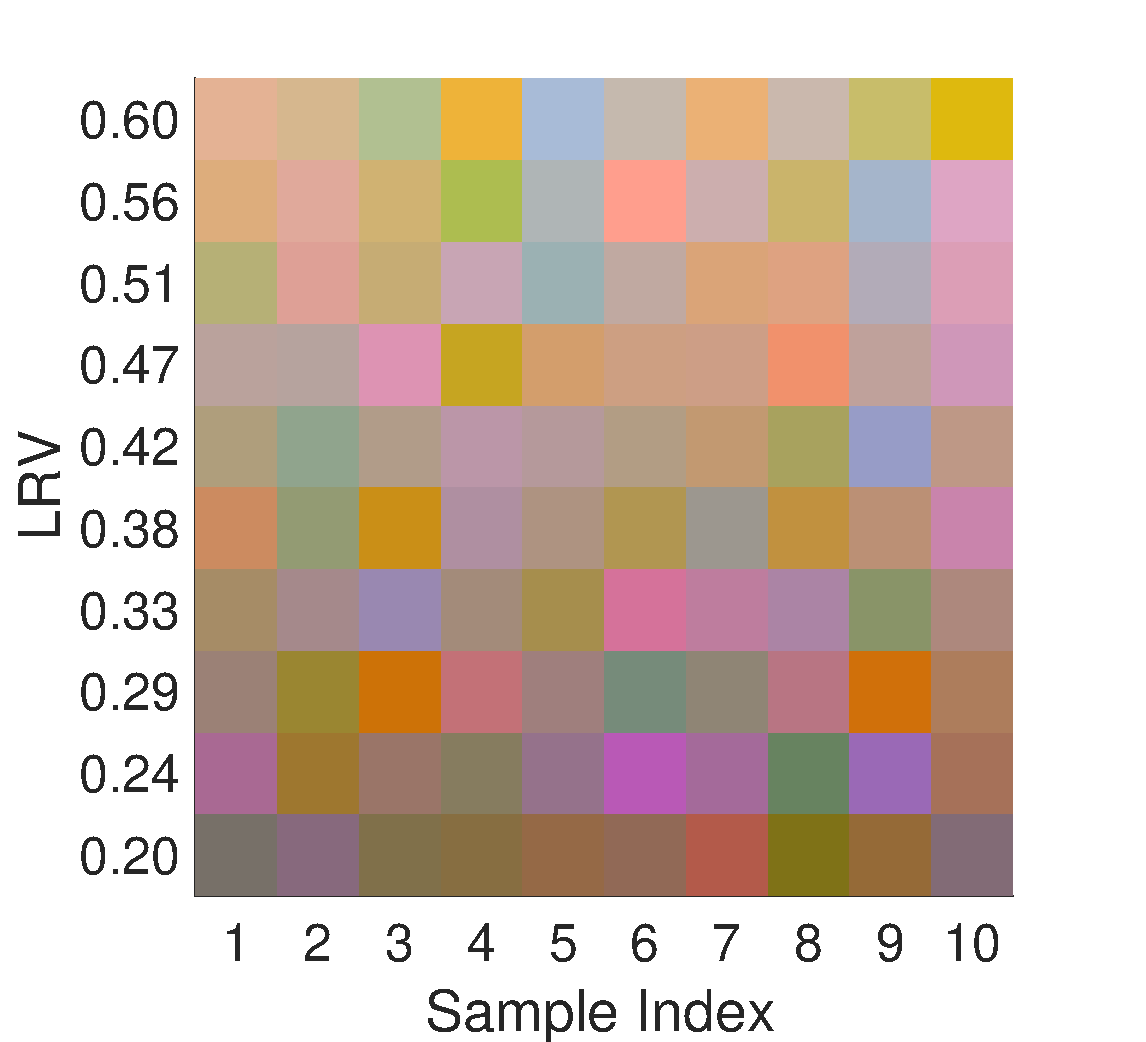
\includegraphics[width=0.3\textwidth]{../Figures/Figure7/Figure8.pdf}
\caption{{\bf Target surface reflectance spectra:} sRGB renditions of the target object surface reflectance rendered under CIE D65 daylight spectrum. The figure shows 10 random samples at 10 equally spaced LRV levels in the range [0.2, 0.6]. This range captures more than 90\% of the natural surface reflectances. Each row contains 10 random samples of reflectance spectra generated at the LRV shown on the left.}
\label{fig:targetSwatches}
\end{figure}


We generated random reflectance spectra using the same principles we applied to generate random illuminant spectra.
We combined the Munsell \cite{kelly1943tristimulus} and Vrhel \cite{vrhel1994measurement} surface reflectance 
measurements to create a database containing 632 reflectance spectra Figure~\ref{fig:reflectanceSpectra}.
The Munsell database contains 462 spectra each measured at 5nm sampling intervals between 380nm and 780nm.
The Vrhel dataset contains 170 spectra measured at 2nm sampling between 390nm and 730 nm.
We resampled these spectra to 31 evenly-spaced wavelengths between $400$nm and $700$nm.
Figure~\ref{fig:reflectanceSpectra} illustrates the spectra of draws obtained using this procedure.
Details of the statistical model for surface reflectance spectra are provided in the appendix. 

% MAKE TARGET SWATCHES ITS OWN FIGURE.
For generating the target object reflectance at a particular luminance $(Y_{\rm T})$, the values in a generated spectrum were 
scaled such that the LRV had the desired value (see appendix).
Figure \ref{fig:targetSwatches} shows color swatches of target reflectance spectra rendered under CIE illuminant D65, for evenly spaced LRV values.

% Figure 8: Methods
\begin{figure}
\centering
\begin{subfigure}[b]{0.25 \textwidth}
		\centering
        \caption{sRGB rendering of a 3D scene}
        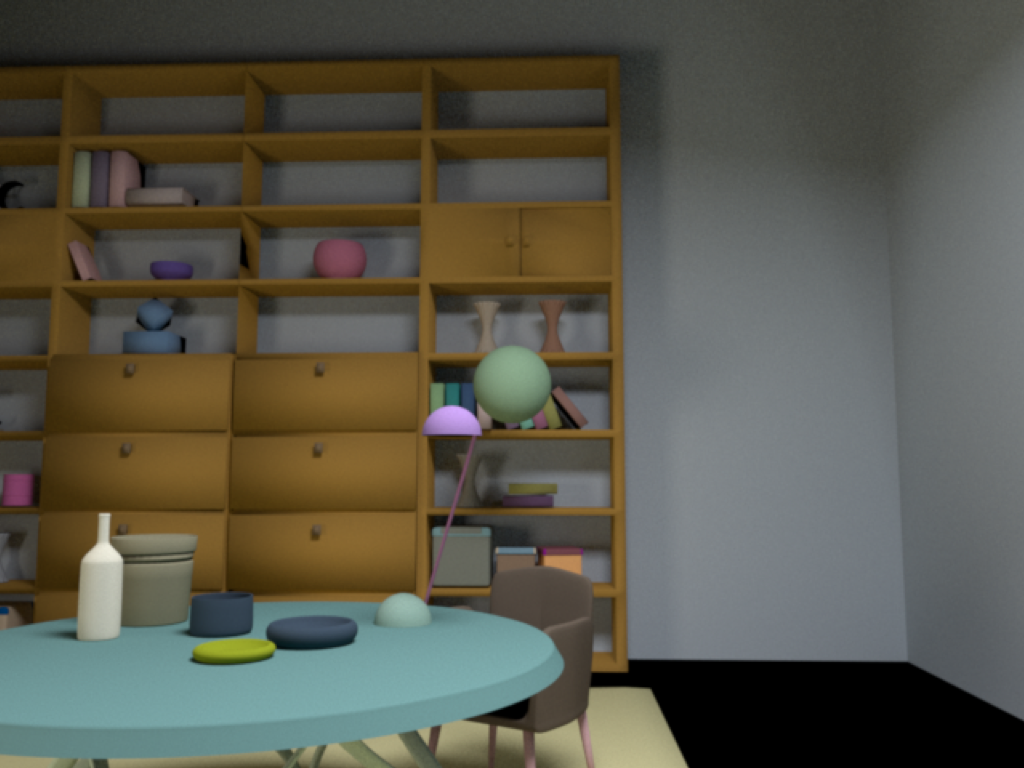
\includegraphics[width=\textwidth]{../Figures/Figure8/Figure8_a.png}
        \label{fig:3DScene}
    \end{subfigure}
    ~ 
    \begin{subfigure}[b]{0.19 \textwidth}   
    \hspace{0.1 \textwidth}
        \caption{Cropped Image}
        \vspace{1.5mm}
        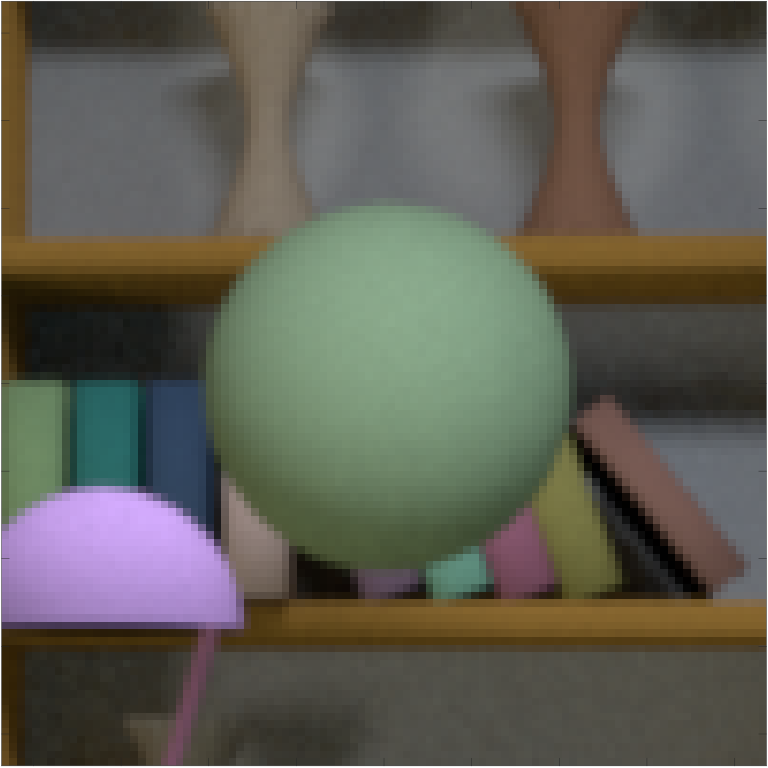
\includegraphics[width=\textwidth]{../Figures/Figure8/Figure8_b.png}
        \label{fig:croppedImage}
    \end{subfigure}
    ~ 
    \begin{subfigure}[b]{0.19 \textwidth}
    \hspace{0.1 \textwidth}
        \caption{Optical Image}
        \vspace{1.5mm}
        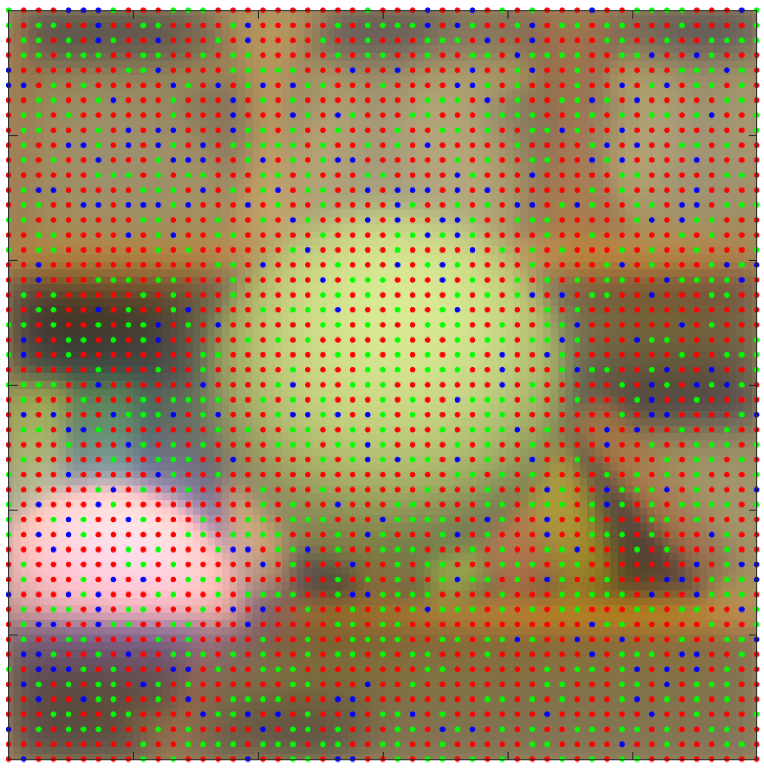
\includegraphics[width=\textwidth]{../Figures/Figure8/Figure8_c.png}
        \label{fig:croppedImageWithMosaic}
    \end{subfigure}
    ~
    \begin{subfigure}[b]{0.2 \textwidth}
        \caption{LMS cone contrast}
        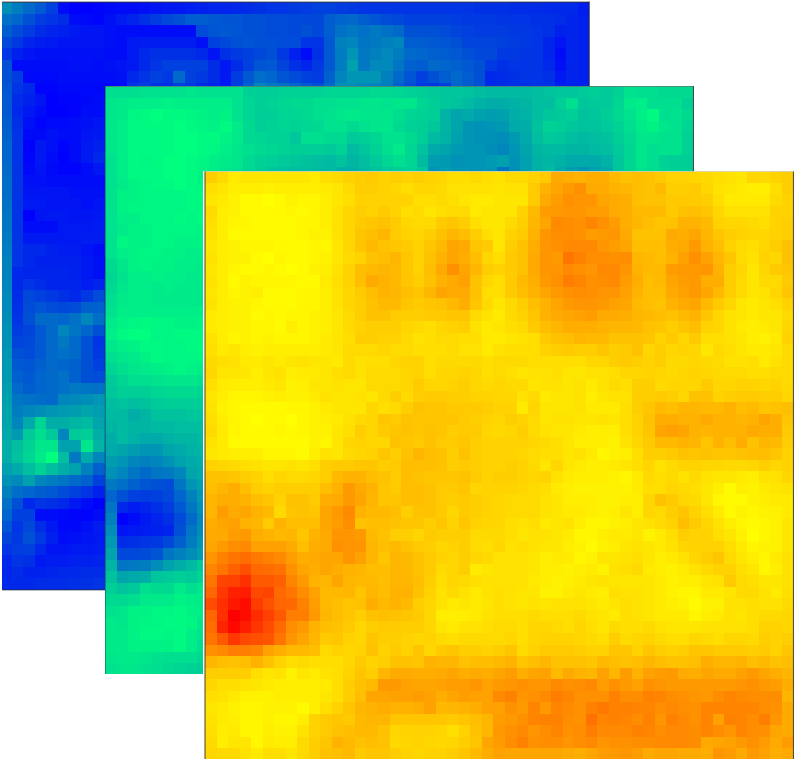
\includegraphics[width=\textwidth]{../Figures/Figure8/Figure8_d.png}
        \label{fig:coneContrast}
    \end{subfigure}
    \label{fig:sceneWithCroppedImage}
    \caption{{\bf Generating labeled dataset for computational analysis:}  For the supervised approach employed in this work, the labeled database is generated as follows: (a) A 3D virtual scene, containing a target object of known surface luminance is created. The target object is placed in the camera field of view. After assigning spectra to the light sources and other other objects in the scene, a multispectral image of the scene is rendered using the Mitsuba software package. (b) The central portion of the rendered image, which contains the target object, is cropped from the image. (c) The retinal image incident on the cone mosaic after optical blurring and the location and the identity of the cones (L cones: Red, M cones: Green, S cones: Blue).  (d) The cone responses are interpolated to estimate the responses of all the three types of cone at each location (demosaicing). Finally, the demosaiced images are contrast normalized separately for each cone type.}
\end{figure}

\subsection{Model of early visual system} \label{method:Isetbio}

The light entering the eye is blurred by the eye's optics.
The resulting retinal image is sampled by a mosaic of cone photoreceptors.
The responses of these photoreceptors provide the information about the scene that is available to the neural visual system for further processing.
Because we are interested in how well luminance constancy may be achieved by the human visual system, we simulated the cone responses
to our scenes using a model of the early visual system.

We focussed our analysis on regions of the image local to the target by cropping the rendered images to $1 \times 1$ degrees of visual angle around the target object ($51 \times 51$ pixels; Figure~\ref{fig:croppedImage}).
This choice is motivated by the observation that neural receptive fields early in the visual pathways (e.g., retina, primary visual cortex) pool information locally.
In foveal primary visual cortex, receptive fields have a spatial extent of approximately 1 degree of visual angle (REFS).
% Johannes to provide his favorite citation or two.  Some review.

We modeled a visual system with a pupil diameter of 3 mm, optical blurring (including axial chromatic aberration) in the formation of the retinal image (REF whatever optics model), spatial sampling by an interleaved mosaic of long (L), middle (M)  and short (S) wavelength-sensitive cones (Brainard mosaic review; Fig.~\ref{fig:croppedImageWithMosaic}). The cone mosaic contained  L:M:S cones in the ratio 0.6:0.3:0.1 and with spectral sensitivities derived from the CIE physiological standard (REF).
Cone isomerizations were computed assuming an integration time of 5 msec, and we modeled the Poisson nature of photopigment isomerization (REF Hecht et al). This modeling was implemented using the software infrastructure provided by ISETBio (REF).

% Details from Nicolas (TEXT IN CAPS IS FROM VIJAY)
% Scene: 
%- the default mean luminance was set to 200, but there is a key-value param that could have overriden this value. 
%  I do not know if this were the case.
%
% % MEAN LUMINANCE = 0, NO SCALING

%- The default FOV was 1 deg, but there is a key-value param that could have overriden this value.
%  I do not know if this were the case.
%
% % HORIZONTAL FOV = 1

%- Distance default is 1 meter, but there is  a key-value param that could have overriden this value.
%  I do not know if this were the case.
%
%% DISTANCE 1M

%
%Optics: 
%- 3 mm pupil, 17 mm focal length, with a spectro-spatial OTF described in  
%  (Marimont & Wandell (1994) J. Opt. Soc. Amer. A,  v. 11, p. 3113-3122), 
%   which includes axial chromatic aberration. However, there is key-value param o skip the OTF. 
%   Not sure if this was used.  It it was used, the optics was set to diffraction limited.
%
% % SKIP OTF OFF:  'skipOTF', false ...  

%
%Lens: 
%- not sure if the optical density is from Wyszecki&Stiles or from Stockman-Sharpe. 
%  The isetbio file commend only says it is from PTB. David do you know, or should I check
%  the data?
%
%Cone Mosaic: 
%- rectangular cone mosaic with 0.6:0.3:0.1 LMS densities
%- FOV was a key-value param, so I do not know what was used.
%- Also the mosaic was subsampled  according to a cone-stride param, with a default of 15 cones
%but there is a key-value param that could have overriden this value. I do not know what that parameter value was.
%
% CONE STRIDE = 3 'coneStride', 3, ... 

%
%- There is a key-value pair to also low-pass the optical image with default value to not do so.
%  If that was user-overriden the OI was lowpass filtered using a Gaussian whose sigma was dependent on the cone-stride param.
%
% LOW PASS FILTER = MATCH CONE STRIDE : lowPassFilter = 'matchConeStride';      

%- IntegrationTime was not specified, so it was the default which is 5 msec.
%  The cone isomerization maps were also demosaiced using linear interpolation.
%- The default isomerization noise was set to none, but there is a key-value parameter
%  that can override it. I do not know what the value of that was.
%
% ISOMERIZATION NOISE = FROZEN, 'isomerizationNoise', 'frozen'

%-  Finally, there is a key-value param named 'coneEfficiencyBasedReponseScaling', which by default is set to 'none'
%   But if it was user-set to non 'none' the code scaled the responses to simulate equal quantal efficiencies 
%   for L , M and S coneEfficiencyBasedReponseScaling by undoing filtering by the lens and the macular pigment.
%   I do not know if this was used.
% 
% coneEfficiencyBasedReponseScaling = 'area'


The cone isomerizations represent the first step of visual processing.
To capture key properties of post-receptoral processing, such as contrast normalization \cite{heeger1992normalization,albrecht1991motion,carandini2012normalization},
we processed the isomerizations as follows:
First, we generated a response for each cone class at each pixel in the sampled retinal image, using bilinear interpolation separately for each cone class.
This gives us a cone response image for each cone class.
We also normalized each cone response image by the total area under the corresponding cone spectral sensitivity.
This makes the magnitude of the cone response images similar across cone classes.
These two processing steps do not alter the information in the cone response images. 

To model contrast coding, we converted each cone response image to a corresponding cone contrast image.
This was accomplished by computing the mean response over the three cone contrast images, and then subtracting off and dividing by this mean.
To model contrast normalization, we divided by the sum of squared contrasts over image pixels and cone classes.

%The sampling and rendering steps described above allow us to generate images from scenes that contain an image of a target object of known surface luminance at the center pixel, and where the illuminant spectra and spectra of the other surfaces in the scene are drawn randomly from models of naturally occurring spectra.  One such image is shown in Fig.~\ref{fig:3DScene}, where the green sphere in the middle is the target object and the light sources are not within the camera field of view. We model the encoding of such images by the early visual system, to generate {\em neural images} that provide an abstracted representation of the information available to the brain for producing perceptual representations of the external world. For each image, it is this information together with the known surface luminance of the corresponding target object that we will provide to our supervised learning algorithms.  Our training datasets correspond to ... % SAY WHAT WE DID ONCE WE FINISH EVERYTHING OFF.

% NEED TO WRITE IN THE KEY PARAMETERS USED. PROBABLY MARIMONT AND WANDELL OPTICS, STOCKMAN-SHARPE LMS CONE SPECTRAL SENSITIVITIES, THE L, M, S CONE RATIO IN THE MOSAIC, RECTANGULAR AND REGULAR CONE PACKING, SOME IMPLIED SPATIAL SCALE, AND SOME OVERALL SCALING THAT DRIVES THE MEAN LUMINANCE OF THE RETINAL IMAGES AND THUS THE AMOUNT OF POISSON NOISE. ALSO INTEGRATION TIME.

% NEED TO UNDERSTAND THIS.  WHEN WAS THE GAIN, BEFORE OR AFTER NOISE ADDED, AND LET'S REMEMBER WHY WE DID IT.  
% First we add noise, then we do the scaling. The reason this was done is to make sure that in the normalization process each of the cone class have the same contribution. Otherwise, the S cone contribution would be very low.

\subsection{Computational luminance constancy} \label{method:SupervisedLearning}
We used our datasets to determine how well target object LRV can be estimated from cone responses and from normalized cone contrasts.
Studying both representations allows us to understand how early contrast coding and normalization affect how well luminance constancy can be achieved.
We applied accuracy maximization analysis (AMA) to learn the optimal receptive fields for estimating LRV,
and evaluated the performance obtained when the output of these filters was optimally decoded.

\subsubsection*{Learning optimal filters}

AMA \cite{geisler2009optimal,burge2017accuracy,jaini2017linking}
is a task specific Bayesian method for dimensionality reduction.
When provided with a labeled training set, a receptive field response model, a decoder that uses these responses to estimate the stimulus label, and a cost function, AMA returns a set of linear receptive fields.
These receptive fields have the property that the  expected estimation cost is minimized when their responses are optimally decoded.

More concretely, let us assume that there are $N_{\nu}$ possible values of the target LRV levels ($\{Y_k: k\in[1,N_{\nu}] \}$) and the $l$'th image corresponding to the $k$'th luminance level is represented as $s_{kl}$. Also, assume that there is a set of linear receptive fields {\textbf{\textit f}} which when acting on $s_{kl}$ gives the response ${\textbf{\textit R}}_{kl}$. Also assume there is a decoder $g$, with the knowledge of the response model and of every stimulus in the training set, that returns the Bayes' optimal estimate of the luminance level ($\hat{Y}_k$) of the target object in each stimulus $s_{kl}$. The crux computation for obtaining this estimate is the computation of the posterior probability of the luminance given an observed response, $P(Y|\textbf{R}_{kl})$ \cite{geisler2009optimal,burge2017accuracy,jaini2017linking}
. With this luminance estimate, we calculate the cost given the cost function $\mathcal{C}_{kl} = \gamma(Y_{kl},\hat{Y}_{kl})$. Finally, AMA searches for the set of optimal receptive fields ${\textbf{\textit f}}^{\rm opt}$ that minimize the cost over the entire training set $\{s_{kl}: k\in[1,N_{\nu}], l\in[1,N_k]\}$ where $N_{k}$ is the number of stimuli corresponding to the label $Y_k$. Thus,
\begin{align}
{\textbf {\textit f} }^{\rm opt} = \argmin_{\textbf {\textit f} } \sum_{k=1}^{N_{\nu}}  \sum_{l=1}^{N_k} {\mathcal{C}}_{kl}.
\label{eq:fopt}
\end{align}

\subsubsection*{Decoding optimal filters}

Once the optimal receptive fields have been learned, a general decoder must be used to estimate the luminance. Recall that the decoder used to learn the receptive fields required the knowledge of every stimulus in the training set. To obtain the general decoder, first we use the AMA optimal receptive fields and the training dataset to find the conditional distributions of the AMA receptive field responses $P({\textbf {\textit R} }|Y_i)$. Then, we approximate these with multivariate Gaussian distributions $P({\textbf {\textit R} }|Y_i) = \mathcal{N}\left(\mu(Y_i),\Sigma(Y_i) \right)$. To estimate the luminance of the target object in the test stimulus, we use Bayes' rule to obtain the posterior distribution $P(Y|{\textbf {\textit R} })$. The optimal estimate is the luminance value that minimizes the cost function.

\subsubsection*{Baseline performance measure}

We used linear regression to provide a baseline performance measure.

Linear regression gives us a baseline estimate of the performance. We use this method to estimate the target object LRV using cone responses corresponding to the central pixel of the cropped image. Thus, getting an estimate for a condition that does not take into account the context in the scene. 

For for linear regression, we solve the set of linear equations given by $A_{1\times3}*C_{3\times N} = Y_{1\times N}$ for the regression parameters $A_{1\times3}$. Here, $C_{3\times N}$ is a matrix containing the average L, M and S stimulus of a central  3$\times$3 pixel patch of the image. We use Matlab to obtain the (unknown) regression parameters $A$.

\subsection{Performance metric}
If $\hat{Y}$ is the estimated luminance corresponding to the assigned luminance $Y$, the error of the luminance estimates is quantified as the relative error ($E_{\rm rel}$) defined as: $E_{\rm rel}^2 = \left\langle\left((\hat{Y}-Y)/Y\right)^2\right\rangle$.


% THINGS TO THINK ABOUT:
%  1) Putting error bars on performance.  Particularly want to be sure that Fig 13 feature that Condition 3 RFs do better than Condition 1 RFs for Condition 1 is just statistical sampling.

\section{Results} \label{Results}
In this section, we discuss the results of supervised learning to estimate the luminance of the target object on the conditions we described previously. We describe the computations that need to be performed on the cone photoreceptor responses to estimate the luminance. We start with condition 1, where only the reflectance spectrum of the target object is allowed to vary, and show that in this condition the luminance can be estimated directly from the photoreceptor response. We then progressively increase the complexity of the spectral conditions and explain the correspondingly complex computations that are required to estimate the target LRV. Next, we show the optimal AMA receptive fields for each one of the spectral conditions discussed in this work. We show that the optimal receptive fields for target luminance estimation have a center surround structure and they give more weights to the response of L and M cones than S cones. We finally show that, as expected, the receptive fields for the complex spectral conditions generalize to the simple conditions. Hence, one requires only one set of optimal receptive fields for estimating the target luminance, not separate receptive fields for each spectral condition.

\subsection{Luminance estimates for each spectral condition}
\subsubsection{Condition 1: Target object relative surface reflectance spectrum variable, light source and background object spectra fixed}
We start with the results of the simplest type of spectral variation where only the target object relative surface reflectance spectrum is allowed to change. 
We used AMA to learn a set of linear receptive fields that are optimal for estimating target LRV from the model cone photoreceptor response to the images from this condition.
Fig.~\ref{fig:case1RFResponse} shows the projection of the photoreceptor response along the first two optimal AMA receptive fields. 
Clearly, there exists a subspace along which the photoreceptor response separates according to the luminance level assigned to the target object. 
Thus, the target LRV can be obtained by projecting the photoreceptor response along these AMA receptive fields. 
We used such projections and a generalized Bayes' decoder (see methods) to estimate the luminance of the target objects in the test set stimuli. 
Fig.~\ref{fig:case9Results} shows the estimated luminance v/s the actual luminance assigned to the target object for the test stimuli in condition 1. 
We show the estimates obtained by AMA and two null models: a naive method that assigns the average target LRV across the training set to all images, and a linear model based on the photoreceptors corresponding to the center pixel on the target object (see Methods). 
As expected, in the absence of any external source of variation, the photoreceptor response is proportional to the luminance of the target object, and hence can be easily estimated by both AMA and linear regression.

Each cloud in Fig.~\ref{fig:case1RFResponse} corresponds to the photoreceptor response to the images with target luminance level at a fixed value. 
The variation within the cloud, between images that have the target object at same luminance values, is due to the difference in the relative shape of the target object reflectance spectra (difference in hue and saturation). 
The resulting variation dominates any variation coming from the noise in photoreceptor response or the noisy rendering of the images by the software.
Fig.~\ref{fig:case0RFResponse} shows the projection of photoreceptor response corresponding to 1000 images where, in addition to the illumination and background spectra, we also fixed the relative shape of the target object surface reflectance. 
The variation resulting from the poisson nature of the photoreceptor response or due the image rendering software is small and can be ignored.

%% Figure 9
\begin{figure}
\centering
        \begin{subfigure}[b]{0.3 \textwidth}
        \caption{RF response condition 0}
        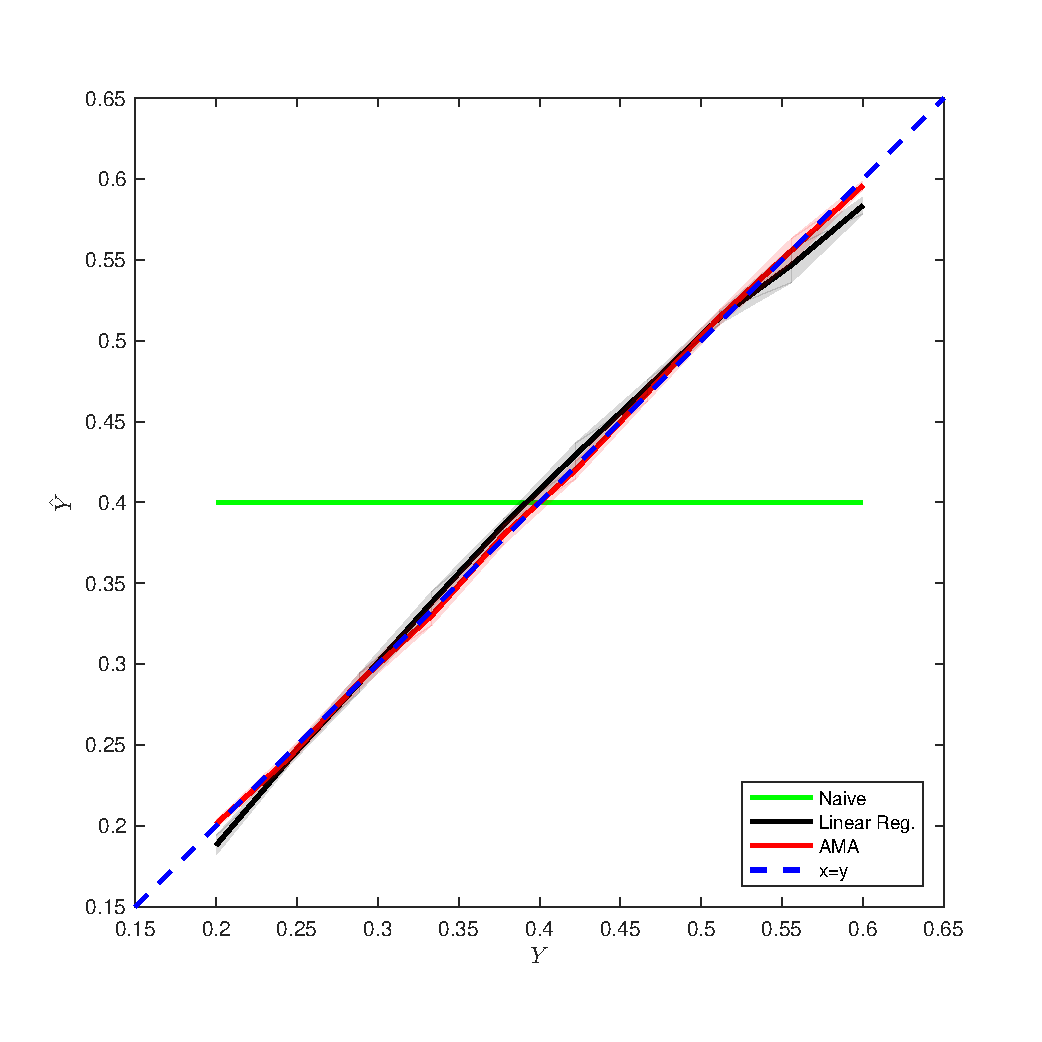
\includegraphics[width=\textwidth]{../Figures/Figure9/Figure9_c.pdf}
        \label{fig:case0RFResponse}
    \end{subfigure}
        \begin{subfigure}[b]{0.3 \textwidth}
        \caption{RF response condition 1}
        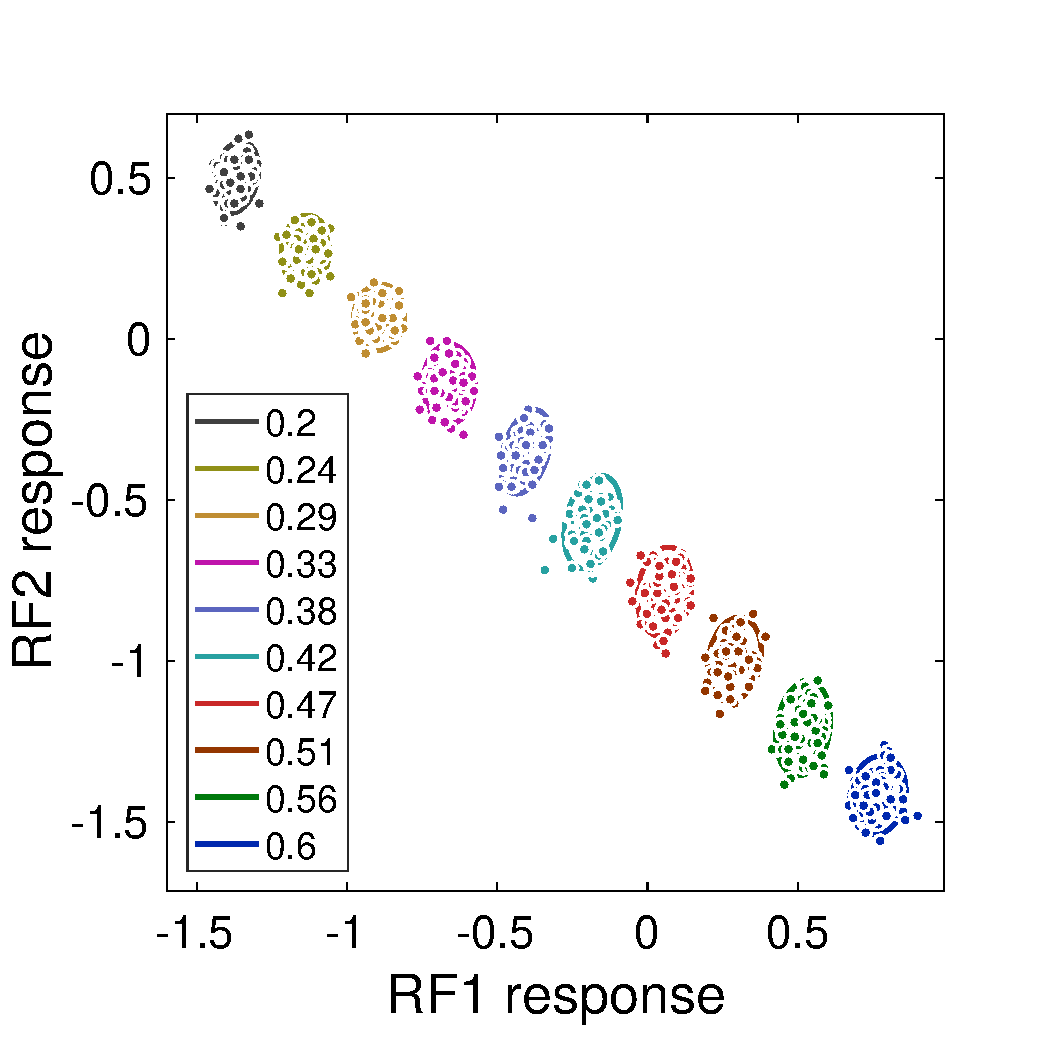
\includegraphics[width=\textwidth]{../Figures/Figure9/Figure9_a.pdf}
        \label{fig:case1RFResponse}
    \end{subfigure}    
%    \begin{subfigure}[b]{0.33 \textwidth}   
 %       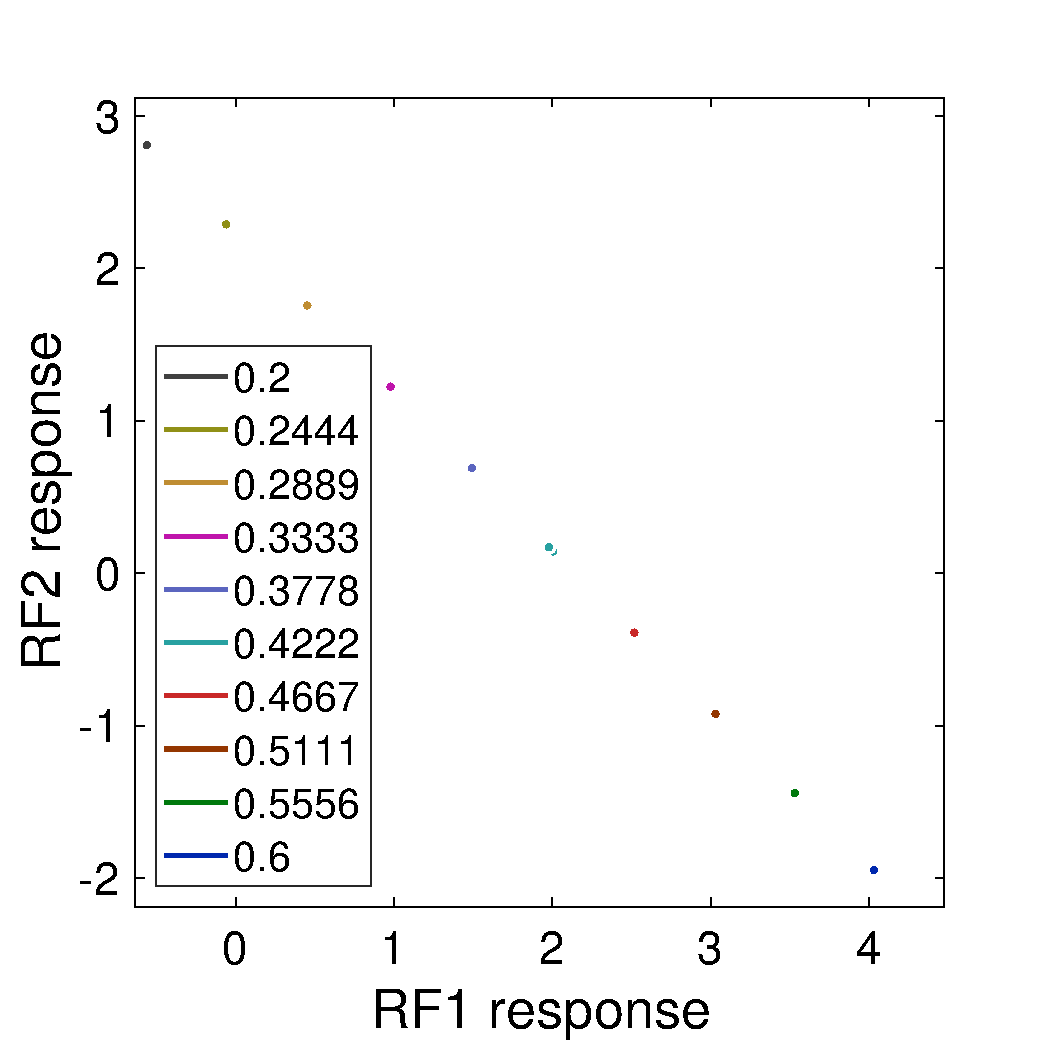
\includegraphics[width=\textwidth]{../Figures/resultsFigure/renderingNoise.pdf}
%        \caption{Rendering noise}
%        \label{fig:renderingNoise}
%    \end{subfigure}
            \begin{subfigure}[b]{0.297 \textwidth}
        \caption{Luminance Estimates}
        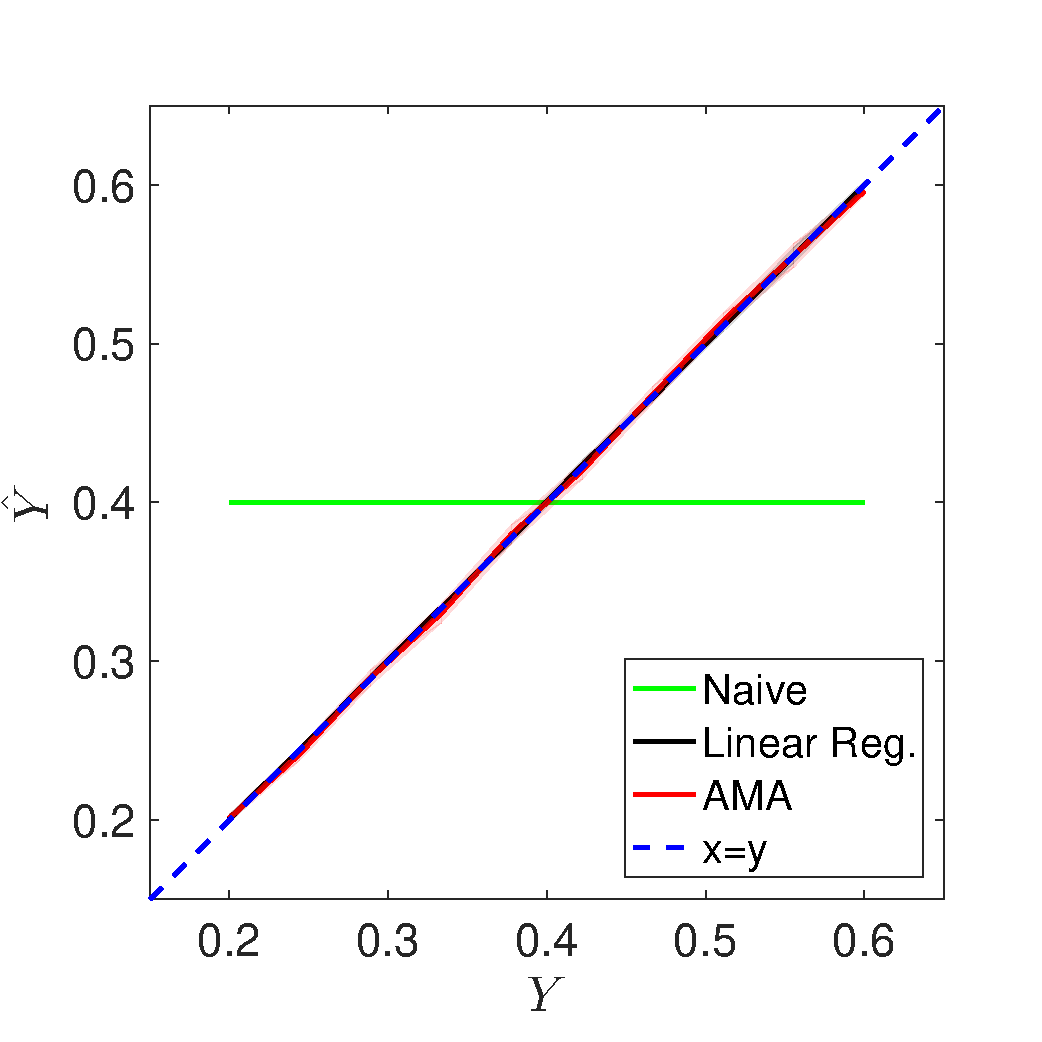
\includegraphics[width=\textwidth]{../Figures/Figure9/Figure9_b.pdf}
        \label{fig:case9Results}
    \end{subfigure}    
    \caption{{\bf RF response and luminance estimates for condition 0 (baseline) and condition 1:} (a) Photoreceptor response projected along the first two AMA receptive fields for images of condition 0. We show the response for the images in the training set. Each response cloud represents the response of images corresponding to one luminance level. The response clouds are approximated by a multivariate Gaussian whose mean and variance are approximated by the ellipses shown in the figure. (b) Photoreceptor response for images of condition 1. (c) Mean luminance estimates and standard deviations for the images in the test set obtained using the naive method, linear regression and AMA. The estimates fall along the diagonal unit slope (blue dotted) line for both linear regression and AMA. The standard deviations are too small to be visible.}
\label{fig:sourcesOfNoise}
\end{figure}

\subsubsection{Condition 2: Target object relative surface reflectance spectrum variable, light source spectra fixed, background object spectra variable}
When the light source emission spectrum is fixed, the naive expectation would be that the luminance of the target object would depend only on the surface reflectance of the target object. 
Indeed, it is believed that the variation in the surface reflectance of the background has little effect on the reflected light from the target object  \cite{BrainardWandellRetinex}. 
But our analysis shows that the secondary reflections from the target object, of the light coming indirectly after being reflected from the background objects, have a significant effect on the response of the photoreceptors corresponding to the target object. 
Fig.~{\ref{fig:case2RFResponse}} shows the projection of the photoreceptor response for the stimuli in condition 2 along the first two AMA receptive fields. 
These receptive fields were learnt using the stimuli from the same condition (Condition 2). 
The response projected along the first two optimal receptive fields do not separate as well compared to condition 1. 
But the overlap is lower if the projection is considered in subspaces that have more AMA receptive fields. 
Fig.~\ref{fig:ErrorVsNFilters} shows the relative error of luminance estimate as a function of the number of AMA receptive fields used for luminance estimation. 
As expected, the relative error decreases with the number of receptive fields and converges to the minimum value around 8 receptive fields. 
Fig.~\ref{fig:case2Estimates} shows the luminance estimates for the learning methods used in this work. 
The mean estimates fall along the diagonal x=y line. 
The variance in the estimates increases with assigned luminance. 
This is because the isomerization noise is directly proportional to the light reflected from the target object and is higher at higher values of the target LRV.

%% Figure condition 2
\begin{figure}
\centering
    \begin{subfigure}[b]{0.3	 \textwidth}   
        \caption{RF response condition 2}
        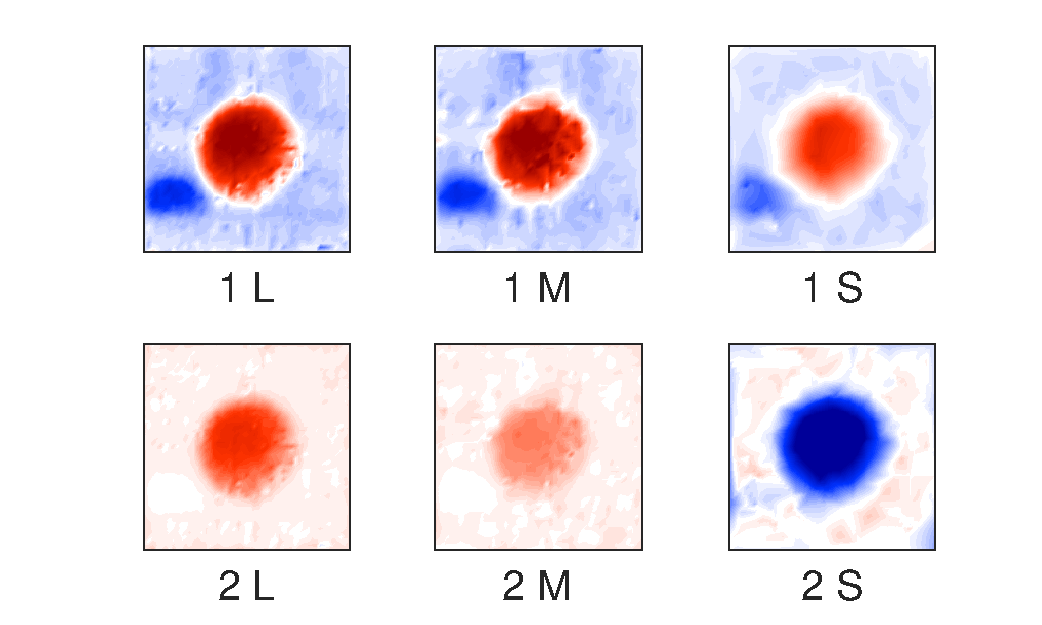
\includegraphics[width=\textwidth]{../Figures/Figure10/Figure10_a.pdf}
        \label{fig:case2RFResponse}
    \end{subfigure}
        \begin{subfigure}[b]{0.3 \textwidth}
        \caption{Luminance Estimates}
        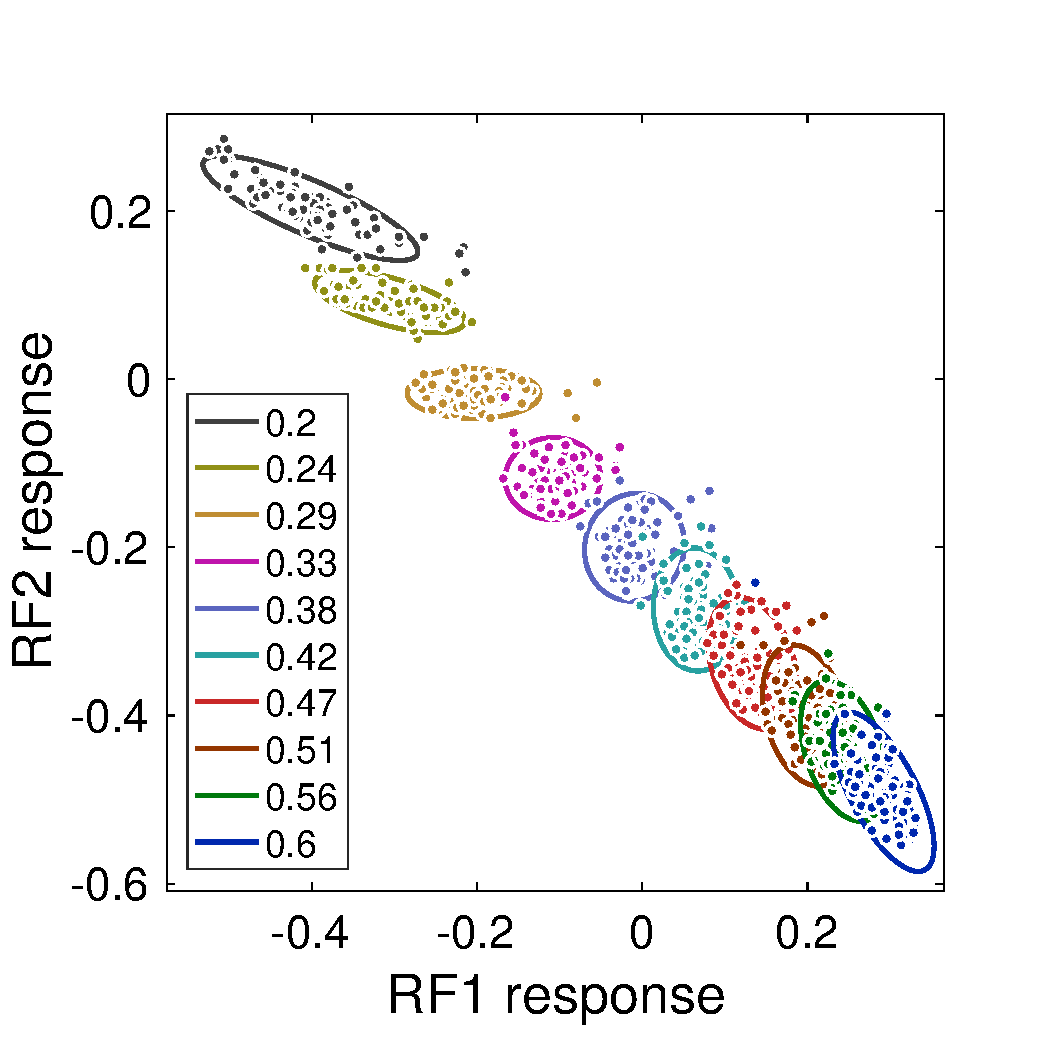
\includegraphics[width=\textwidth]{../Figures/Figure10/Figure10_b.pdf}
        \label{fig:case2Estimates}
    \end{subfigure}
    \caption{{\bf Condition 2:} (a) Photoreceptor response projected along the first two AMA receptive fields. (b) Estimated v/s assigned target LRV for the image in condition 2. Solid lines show the mean estimate, the filled region in light color  shows one standard deviation.}
\label{fig:case2Results}
\end{figure}

%%% Figure 11: RMSE vs N Filters
\begin{figure}
\centering
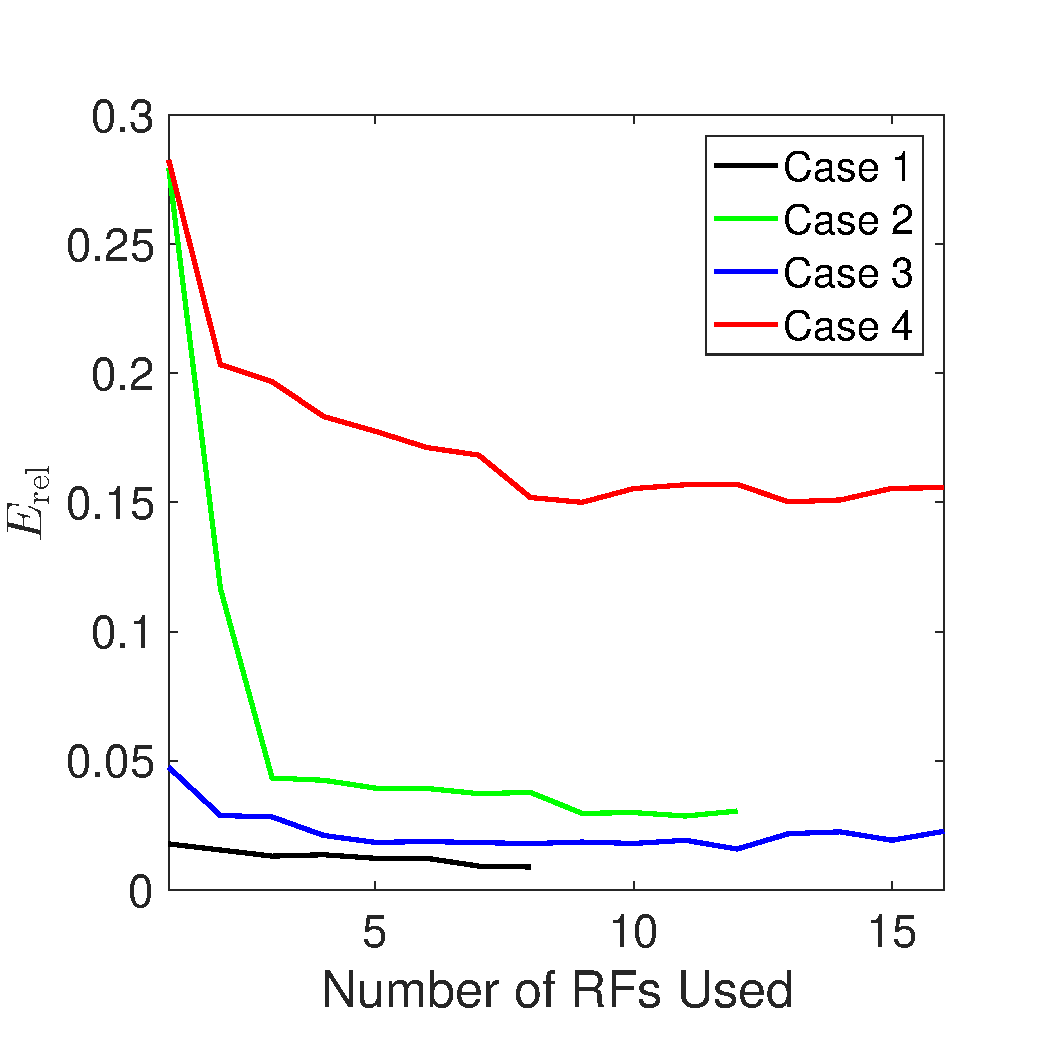
\includegraphics[width=0.3\textwidth]{../Figures/Figure11/Figure11.pdf}
\caption{{\bf Performance with number of RFs used for estimation:} Relative error as a function of number of AMA receptive fields used for luminance estimation. While most of the information is captured by the first two filters, the relative error reduces as the number of receptive fields used for luminance estimation are increased. We have used the first 8 RFs for estimating the luminance.}
\label{fig:ErrorVsNFilters}
\end{figure}

\subsubsection{Condition 3: Target object relative surface reflectance spectrum variable, light source spectra variable, background object spectra fixed}
For the spectral variations of condition 3, the AMA receptive fields learnt on the photoreceptor response to the images does a very poor job in predicting the target LRV (Fig.~\ref{fig:isomerizationFails}). 
This is because, since the illuminant spectra varies in this condition, the photoreceptor response is not directly proportional to the target object surface anymore. 
But, since the background surfaces are fixed in this condition, the ratio between the response of  photoreceptors corresponding to the target object and the background remains proportional to the target LRV. 
This is because a change in illuminant spectra produces the same effect in both the target object and the background object. 
Thus, the AMA receptive fields learnt on the contrast normalized photoreceptor response (see Methods) can be used to predict the target LRV (Fig.~\ref{fig:constrastWorks}). 
Fig.~\ref{fig:case10Results} shows the estimated target LRV v/s the assigned luminance for the images in condition 3 obtained using the contrast normalized representation. 
AMA receptive fields provide excellent predictions of the target LRV. 
The predictions are much better compared to that of a linear model that only considers the (contrast normalized) response of the photoreceptors corresponding to the center pixel of the target object.

%% Figure condition 3: Isomerization Fails
\begin{figure}
\centering
    \begin{subfigure}[b]{0.3	 \textwidth}   
        \caption{RFs learnt using photoreceptor response}
        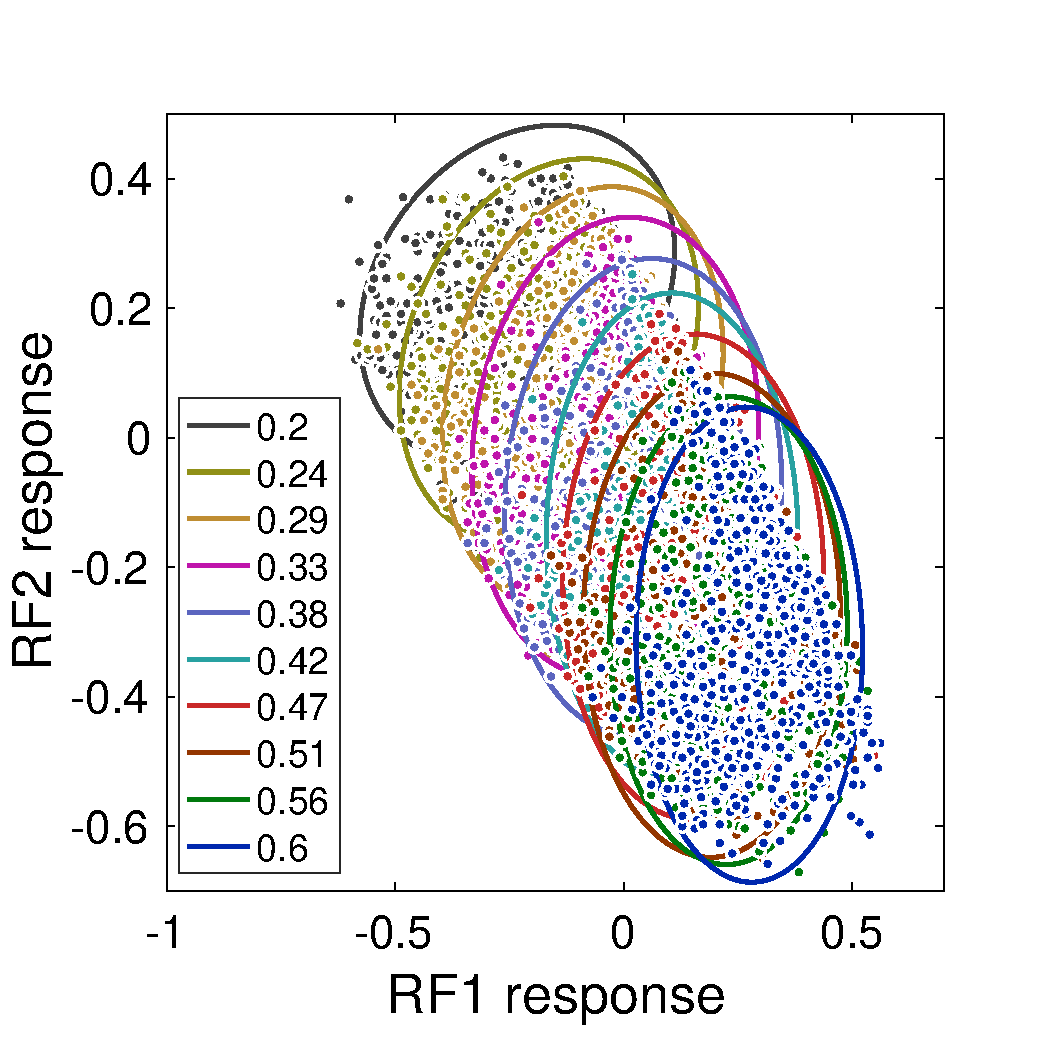
\includegraphics[width=\textwidth]{../Figures/Figure12/Figure12_a.pdf}
        \label{fig:isomerizationFails}
    \end{subfigure}
        \begin{subfigure}[b]{0.3 \textwidth}
        \caption{RFs learnt using contrast signal}
        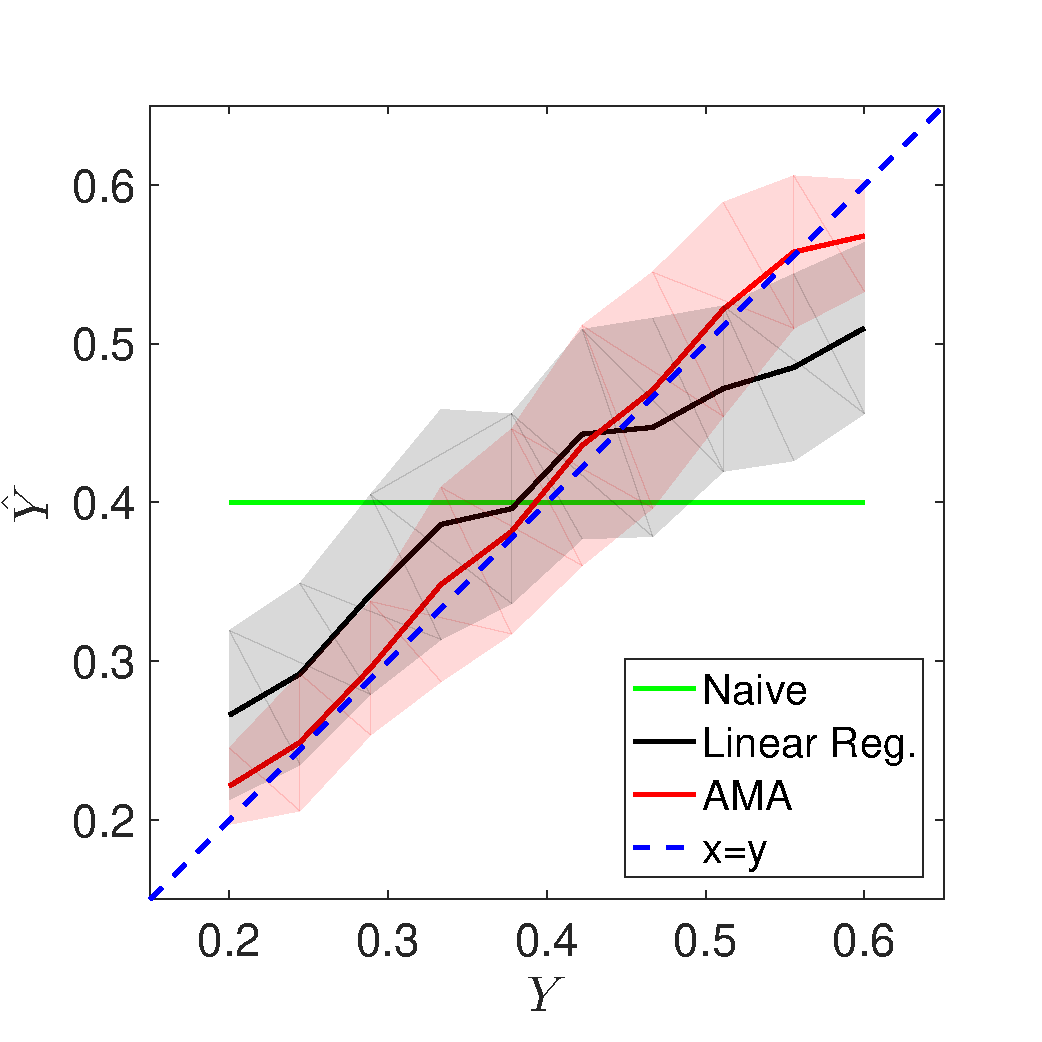
\includegraphics[width=\textwidth]{../Figures/Figure12/Figure12_b.pdf}
        \label{fig:constrastWorks}
    \end{subfigure}
            \begin{subfigure}[b]{0.3 \textwidth}
        \caption{Luminance estimates}
        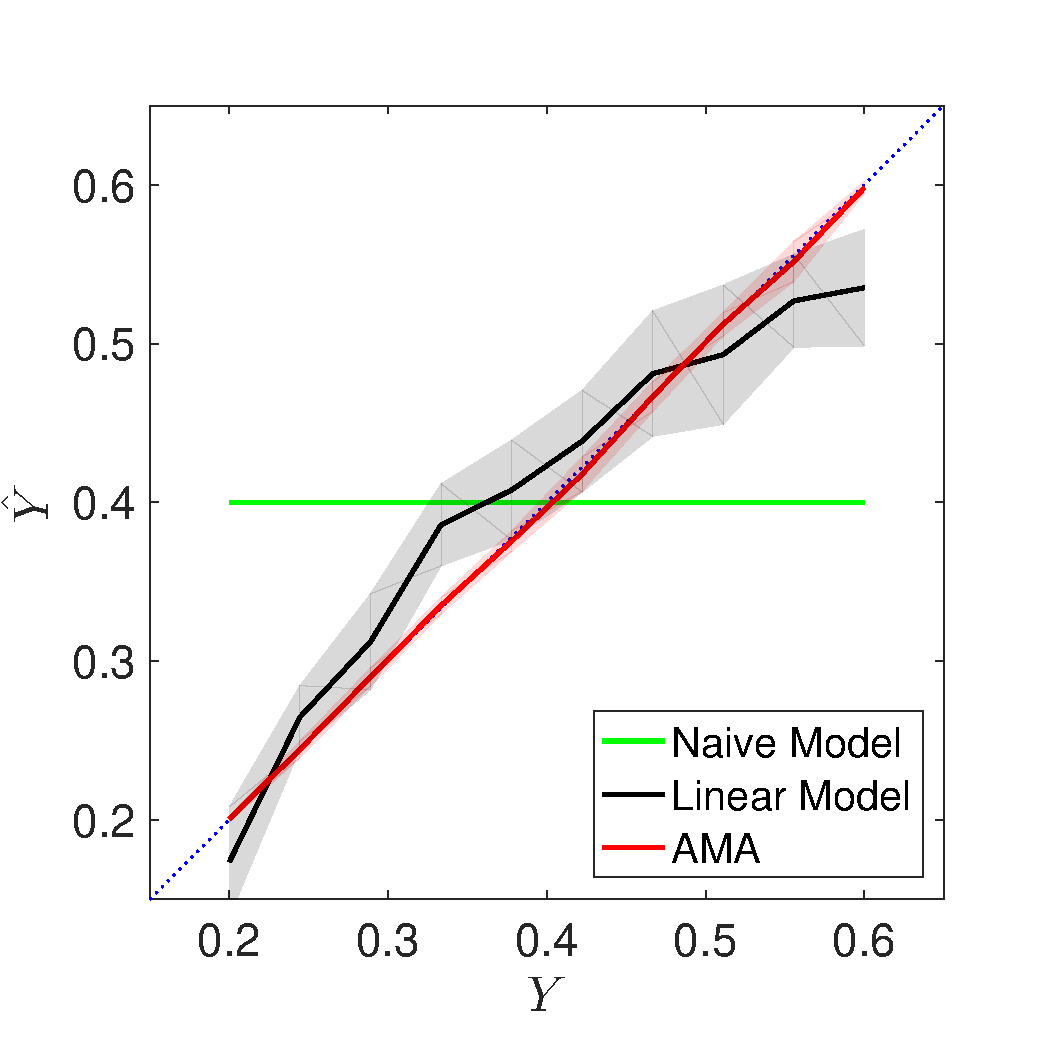
\includegraphics[width=\textwidth]{../Figures/Figure12/Figure12_c.pdf}
        \label{fig:case10Results}
    \end{subfigure}
    \caption{{\bf Condition 3: Luminance can be estimated using the contrast signal:} (a) Photoreceptor response projected on AMA receptive fields calculated using photoreceptor response. (b) The contrast normalized photoreceptor response projected along the first two AMA receptive fields. The receptive fields were calculated using the contrast normalized stimuli. The response at each luminance level separates much better in this representation. (c) Estimated v/s assigned target LRV for the image in condition 3. Solid lines show the mean estimate, the filled region in light color  shows one standard deviation. AMA estimates are much better compared to the null models.}
\label{fig:importanceOfConstrast}
\end{figure}

Again, similar to condition 2, the projection along the first two receptive fields shows an overlap between the stimuli at higher luminance values (Fig.~\ref{fig:constrastWorks}). But, the stimuli are better separated if the projection is considered within a subspace that has more receptive fields (Fig.~\ref{fig:ErrorVsNFilters}).

\subsubsection{Condition 4: Target object relative surface reflectance spectrum variable, light source spectra variable, background object spectra variable}
% Figure condition 4
\begin{figure}
\centering
    \begin{subfigure}[b]{0.3 \textwidth}   
        \caption{AMA RF Response}
        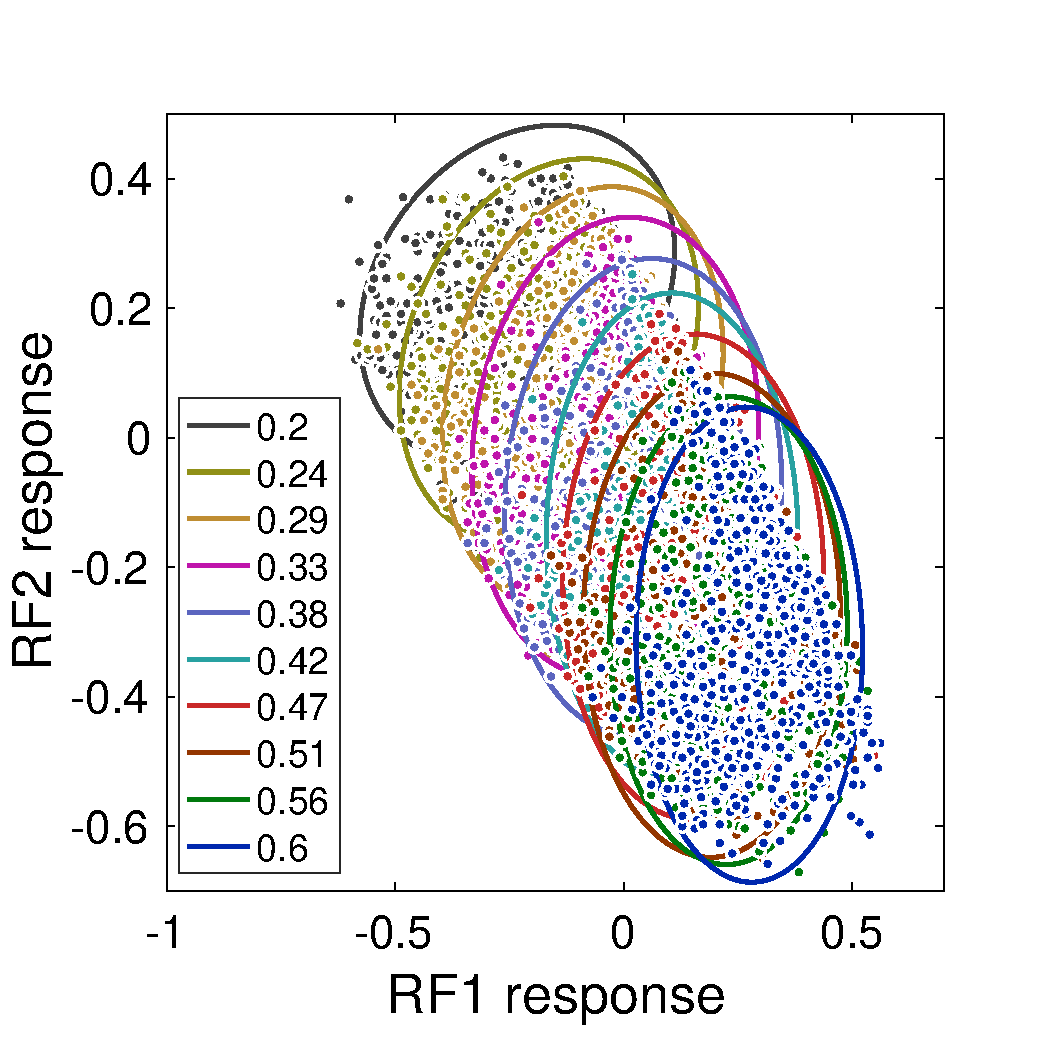
\includegraphics[width=\textwidth]{../Figures/Figure13/Figure13_a.pdf}
        \label{fig:case12FiltersResponse}
    \end{subfigure}    
        \begin{subfigure}[b]{0.3 \textwidth}
        \caption{Luminance Estimates}
        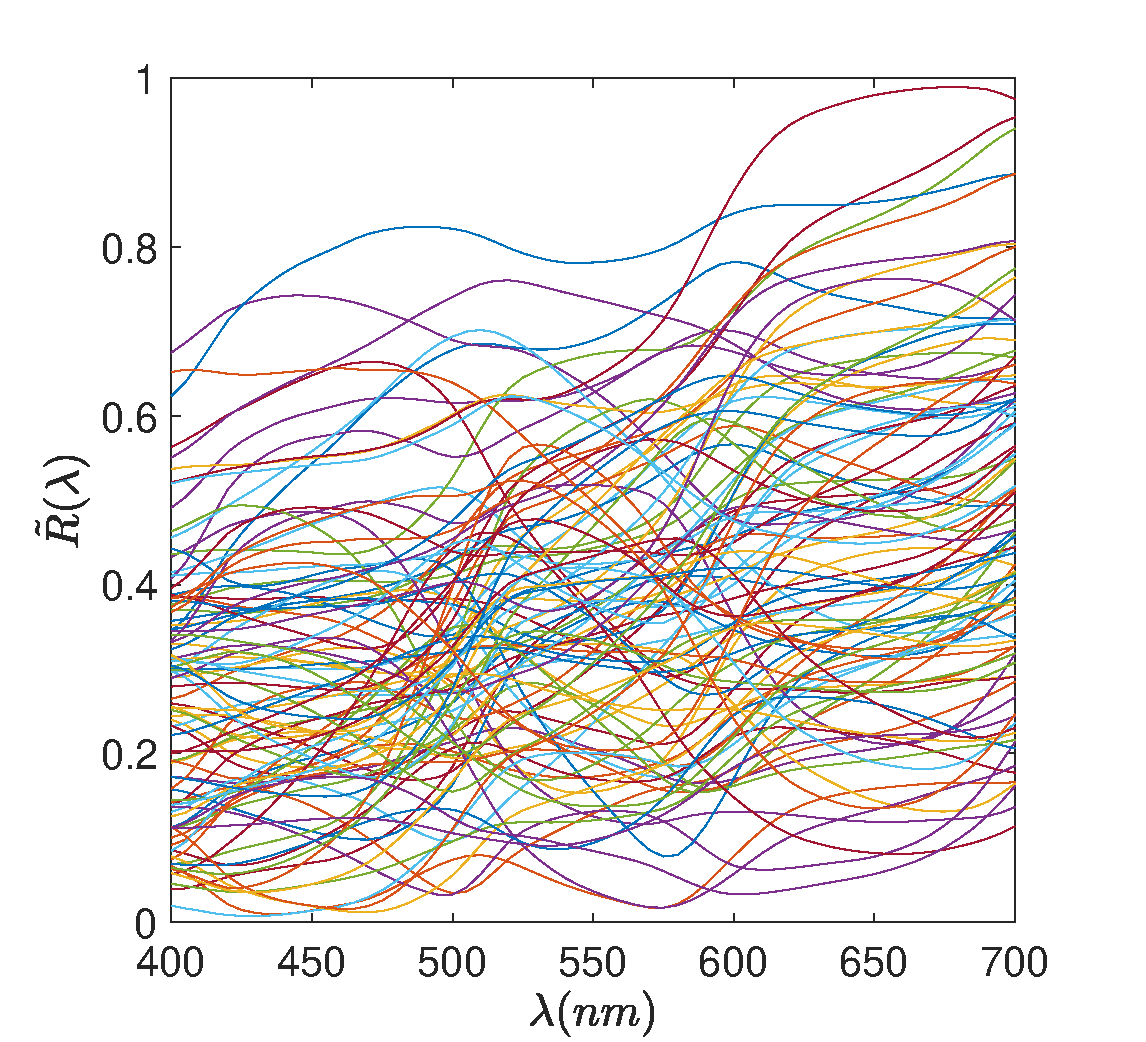
\includegraphics[width=\textwidth]{../Figures/Figure13/Figure13_b.pdf}
        \label{fig:case12Results}
    \end{subfigure}
    \caption{{\bf Condition 3:} (a) Contrast normalized photoreceptor response projected along the first two AMA receptive fields. (b) Target LRV estimates v/s assigned luminance for images in condition 3. The AMA estimates are unbiased and have smaller relative error compared to linear model.}
    \label{fig:case12AllResults}
\end{figure}

Condition 4 is the most complex type of variation that we consider in this work. Here we allow all three types of spectra to change from image to image. In this condition, neither the photoreceptor response (as in condition 1 and 2), nor any simple transformation of the response (condition 3) can provide the target LRV.We used AMA to learn the receptive fields using the contrast normalized cone photoreceptor response from stimuli in condition 4. Fig.~\ref{fig:case12AllResults} shows the AMA receptive field response and the luminance estimates for the images in condition 4. 
We have used the first 8 receptive fields to estimate the luminance in this condition (see Fig.\ref{fig:ErrorVsNFilters}). 
The AMA receptive fields do an excellent job of predicting the target LRV. 
The estimates are unbiased with the mean estimates lying close the diagonal unit slope line (Fig.~\ref{fig:case12Results}). 
The relative error of estimation is $\sim15\%$, which low compared to that of the naive model ($\sim42\%$) or the linear model on center pixel ($\sim21\%$).

\subsection{Optimal receptive fields for luminance estimation have a center surround structure}
% Figure RFs 
\begin{figure}
\centering
\begin{subfigure}{0.21 \textwidth}
	\caption{Condition 1}
	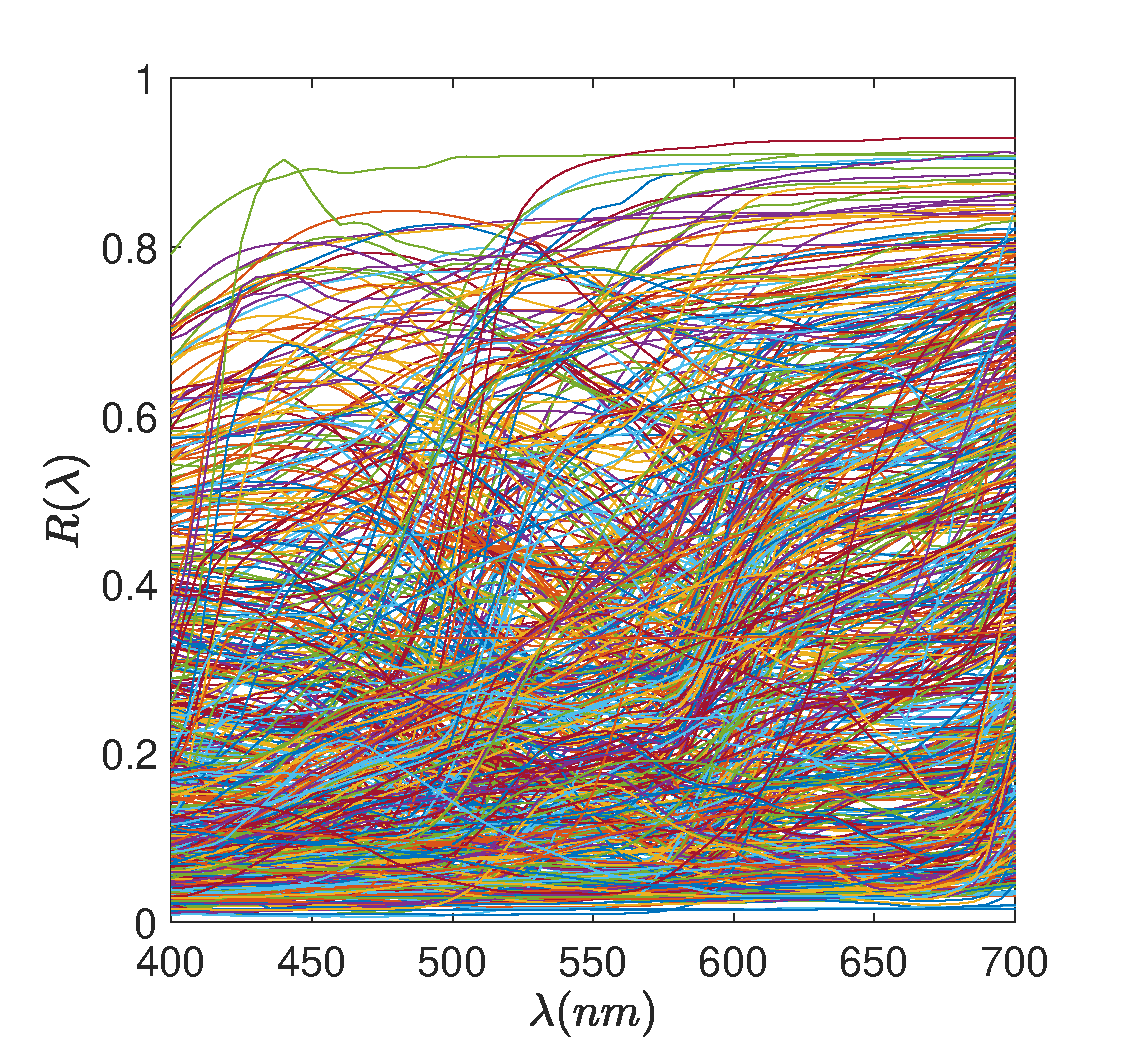
\includegraphics[width=\textwidth]{../Figures/Figure14/Figure14_a.pdf}
	\label{fig:case1Filter}
    \end{subfigure}
    ~ ~ ~
    \begin{subfigure}{0.21 \textwidth}   
	\caption{Condition 2}
	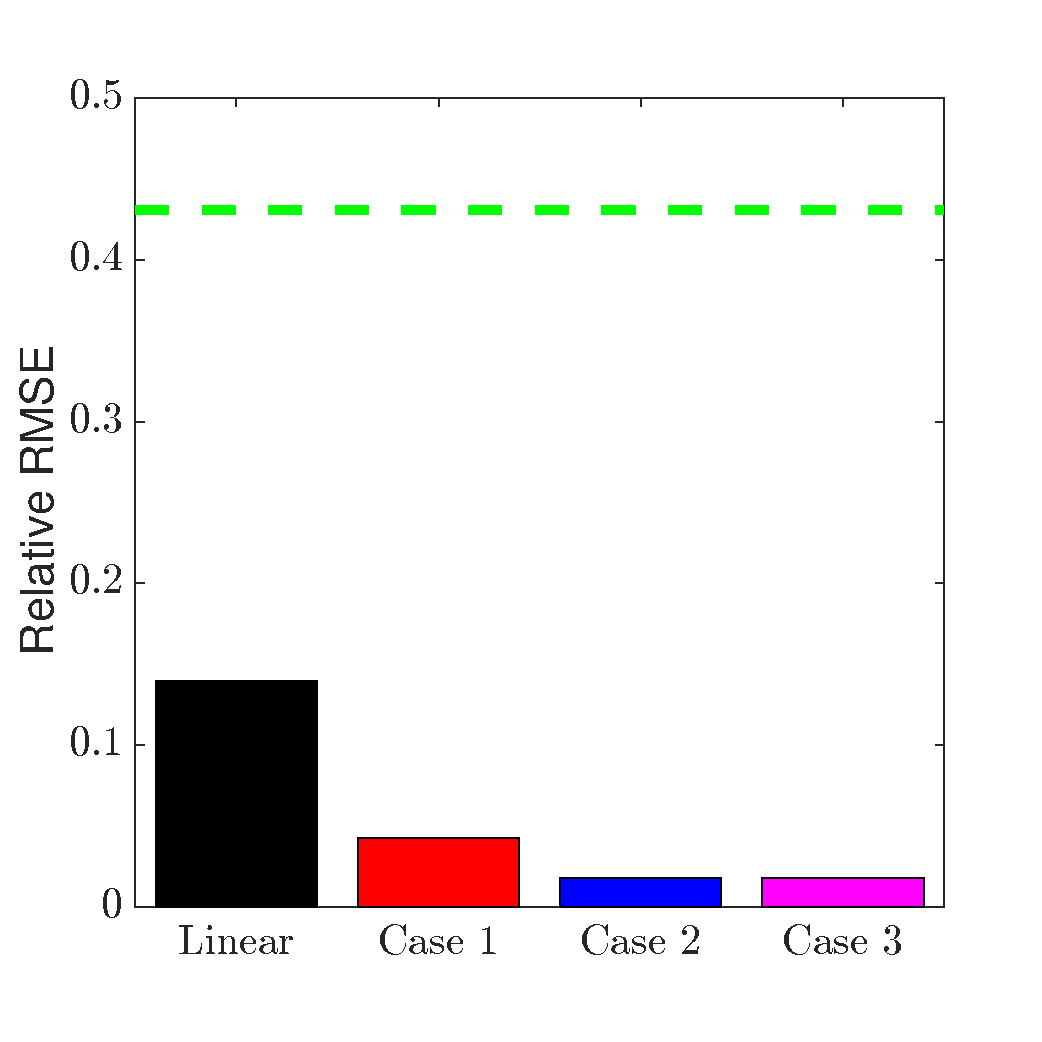
\includegraphics[width=\textwidth]{../Figures/Figure14/Figure14_b.pdf}
	\label{fig:case2Filter}
    \end{subfigure}
    ~ ~ ~
        \begin{subfigure}{0.21 \textwidth}
	\caption{Condition 3}
	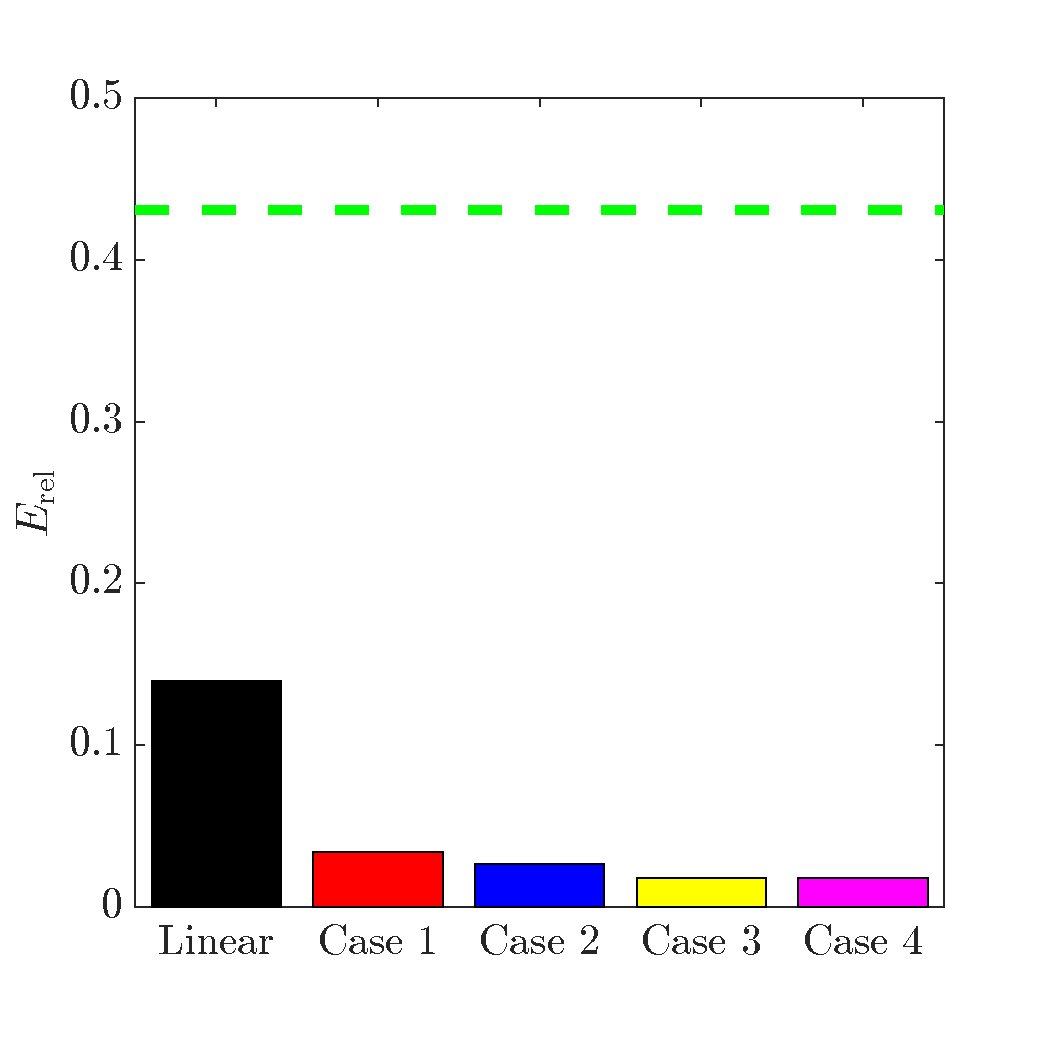
\includegraphics[width=\textwidth]{../Figures/Figure14/Figure14_c.pdf}
	\label{fig:case3Filter}
    \end{subfigure}
    ~ ~ ~
        \begin{subfigure}{0.21 \textwidth}
	\caption{Condition 4}
	\includegraphics[width=\textwidth]{../Figures/Figure14/Figure14_d.pdf}
	\label{fig:case4Filter}
    \end{subfigure}
\caption{{\bf AMA receptive fields:} The first two AMA receptive fields for the four conditions studied in this work. The receptive fields show a center surround structure. The L and M filters have larger weight as luminance is essentially a function of the L and M cone isomerizations. The stereotypical pattern in the receptive fields of condition 4 is due to the fixed geometry of the images.}
 \label{fig:AMAFilters}
\end{figure}

Fig.~\ref{fig:AMAFilters} shows the first two AMA receptive fields that are optimal for estimating the target LRV for the four types of spectral variations studied in this work. The receptive fields are ranked in ascending order of the value of the cost function associated with them. Thus the first RF corresponds to the direction along which the projection of the data gives the minimum cost. The L, M and S components give the weights for the linear sum of the cone responses for the three cone types. The salient features are: the center surround structure of the RFs and the higher weights of the L and M cones, compared to the S cones. 

For condition 1, since the illuminant and the background are fixed, all the information is in the central target object reflectance. Thus, the RFs weights are mostly concentrated around the center. For condition 2, where the target and the background spectra varies, most of the luminance information is still concentrated around the central target object. For condition 3, while the target and the illuminant spectra varies, the background object spectra is fixed. Hence, the luminance can be estimated by simply from the contrast between the response of the cones corresponding to the target and the background. Thus, while the RFs show a trend of weights concentrated at the center similar to condition 1, there is large negative contribution from the surround. The spatial features of the RFs are due the stereotypical geometry of the images (see \nameref{Methods}). Condition 4 has a similar center surround structure, but with more prominent features of the background since the spectra of the background objects are also varying. Again, the spatial features are a result of the stereotypical geometry of the images.

\subsection{The receptive fields of complex condition generalize on simpler conditions}
Fig.~\ref{fig:barGraphs} shows the relative error for the estimates of the target LRV obtained using the linear model and AMA. We show the relative error of the estimates obtained using the AMA receptive fields from all conditions. The receptive fields from a more complex condition perform at par on the stimuli from a simpler condition. The optimal AMA estimates are better than that of the linear model.

% Figure Error Bar Graphs
\begin{figure}
\centering
\begin{subfigure}{0.22 \textwidth}
	\caption{Condition 1}
	\includegraphics[width=\textwidth]{../Figures/Figure15/Figure15_a.pdf}
	\label{fig:case1Bar}
    \end{subfigure}
    ~ 
    \begin{subfigure}{0.22 \textwidth}   
	\caption{Condition 2}
	\includegraphics[width=\textwidth]{../Figures/Figure15/Figure15_b.pdf}
	\label{fig:case2Bar}
    \end{subfigure}
    ~ 
        \begin{subfigure}{0.22 \textwidth}
	\caption{Condition 3}
	\includegraphics[width=\textwidth]{../Figures/Figure15/Figure15_c.pdf}
	\label{fig:case3Bar}
    \end{subfigure}
    ~ 
        \begin{subfigure}{0.22 \textwidth}
	\caption{Condition 4}
	\includegraphics[width=\textwidth]{../Figures/Figure15/Figure15_d.pdf}
	\label{fig:case4Bar}
    \end{subfigure}
\caption{{\bf Comparison of optimal RFs across cases:} Comparison of optimal AMA receptive fields from one condition on the images of other cases. Each panel shows the relative error estimates on the same set of images obtained using the receptive fields of the four cases (condition 1-4). (a) Error estimates for images of condition 1. The AMA receptive fields from all three cases perform well in this case. (b) Error estimates for images of condition 2. As expected, the best estimates are provided by the receptive fields of condition 2. (c) Error estimates for images of condition 3. (d) Error estimates for images of condition 4.}
 \label{fig:barGraphs}
\end{figure}

\section{Discussion} \label{Discussion}
In this paper, we studied luminance constancy using naturalistic images. We used a software pipeline called  Virtual world color constancy (VWCC), which was developed for this work, to generate datasets of multispectral images labeled by the luminance of a target object in each image. VWCC creates 2D multispectral images of 3D scenes based on information provided by the user. Such information include the shape of the 3D space, the shape, size, position and material properties of the objects and light sources in the scene. In our work, we assigned these geometrical and spectral properties using random sampling from available databases of natural objects and light sources. Thus, we generated a large database of labeled hyper-spectral images, with naturalistic scene properties, where we have the ground truth information about every surface and light source. Such databases, of even a few images, are nearly impossible to obtain for natural scenes. This is because it is very hard to measure the surface reflectance and the illumination spectrum at every point in a scene, even for well controlled lab environments. 

We used the software generated labeled images in a supervised manner to understand luminance constancy under four types of spectral manipulations (Fig.~\ref{fig:introExampleFigure}-Fig.~\ref{fig:studiedCases}). We found that target LRV can be recovered through simple manipulation of the retinal cone responses for cases where the spectral manipulations are restricted to at most two of the three possible sources of manipulations: the target object surface reflectance, the background object surface reflectances, or the light source illumination spectra. When variations are allowed only in the target object surface reflectance spectrum, or only the target object and the background objects surface reflectance spectra, the luminance can be estimated directly from the response of retinal cone photoreceptors. If the background spectra is fixed, but the target object reflectance spectrum and the light source illumination spectra are varying, the luminance can be obtained from the contrast between the cone response corresponding to the target and the background. When all three spectral variations are allowed simultaneously, one needs additional information to obtain the target LRV. 


Summary

Effect of background. multiple reflection

center surround RFs

LM

\bibliography{references}
\bibliographystyle{jovcite}

\end{document}

